
\documentclass[10pt,a4paper]{article}

\usepackage{amsmath,amsthm,mathtools}
\usepackage{booktabs,longtable,array,tabularx}
\usepackage{geometry}
\usepackage{natbib}
\usepackage{hyperref}
\usepackage{fontspec}
\usepackage{xeCJK}
\usepackage{unicode-math}
\usepackage{sectsty}
\usepackage{enumitem}
\usepackage{graphicx}
\usepackage{float}
\usepackage{xurl}
\usepackage{tikz}
\usetikzlibrary{positioning,arrows.meta,fit,shapes.multipart}

\geometry{top=20mm,bottom=20mm,left=22mm,right=22mm}
% Standard Japanese mathematical-paper typography:
% Japanese body text in Mincho, headings in Gothic, Latin text in Latin Modern,
% and all mathematical symbols in the dedicated Latin Modern Math font.
\setmainfont{Latin Modern Roman}
\setsansfont{Latin Modern Sans}
\setmonofont{Latin Modern Mono}
\setCJKmainfont[BoldFont=HaranoAjiMincho-Bold,ItalicFont=HaranoAjiMincho-Regular]{HaranoAjiMincho-Regular}
\setCJKsansfont[BoldFont=HaranoAjiGothic-Bold]{HaranoAjiGothic-Medium}
\setCJKmonofont{HaranoAjiGothic-Regular}
\setmathfont{Latin Modern Math}
\linespread{1.05}
\allsectionsfont{\sffamily\bfseries}
\XeTeXlinebreaklocale "ja"
\XeTeXlinebreakskip=0pt plus 1pt
\XeTeXlinebreakpenalty=0
\hypersetup{colorlinks=true,linkcolor=blue,citecolor=blue,urlcolor=blue,hypertexnames=false}
\renewcommand*{\theHtable}{\thesection.\arabic{table}}
\graphicspath{{figs/}}
\emergencystretch=2em
\setlength{\parskip}{2pt}
\raggedbottom
\numberwithin{equation}{section}
\numberwithin{table}{section}
\numberwithin{figure}{section}

\makeatletter
\renewcommand*\l@section{\@dottedtocline{1}{0em}{4.0em}}
\renewcommand*\l@subsection{\@dottedtocline{2}{1.8em}{4.8em}}
\makeatother

\theoremstyle{plain}
\newtheorem{theorem}{定理}
\newtheorem{proposition}{命題}
\newtheorem{lemma}{補題}
\newtheorem{corollary}{系}
\newtheorem{assumption}{仮定}

\theoremstyle{definition}
\newtheorem{definition}{定義}
\newtheorem{remark}{注意}
\renewcommand{\proofname}{証明}
\renewcommand{\abstractname}{要旨}
\renewcommand{\contentsname}{目次}
\renewcommand{\refname}{参考文献}
\renewcommand{\figurename}{図}
\renewcommand{\tablename}{表}

\newcommand{\E}{\mathbb{E}}
% Variables remain mathematical italics; named operators and differentials use
% the upright glyphs of the dedicated mathematics font.
\DeclareMathOperator{\Var}{Var}
\DeclareMathOperator{\Cov}{Cov}
\DeclareMathOperator{\CVaR}{CVaR}
\DeclareMathOperator{\VaR}{VaR}
\DeclareMathOperator{\Skew}{Skew}
\DeclareMathOperator{\Proj}{Proj}
\DeclareMathOperator{\Interp}{Interp}
\DeclareMathOperator*{\argmax}{arg\,max}
\DeclareMathOperator*{\argmin}{arg\,min}
\newcommand{\R}{\mathbb{R}}
\newcommand{\F}{\mathcal{F}}
\newcommand{\A}{\mathcal{A}}
\newcommand{\Lop}{\mathcal{L}}
\newcommand{\Hamil}{\mathcal{H}}
\newcommand{\dd}{\mathop{}\!\mathrm{d}}
\newcommand{\one}{\mathbf{1}}
\newcommand{\GH}{\mathrm{GH}}
\newcommand{\MC}{\mathrm{MC}}
\newcommand{\dt}{\Delta t}
\newcommand{\dx}{\Delta x}
\newcommand{\contribbox}[2]{%
\begin{minipage}[t]{0.48\textwidth}\small\textbf{#1}\par #2\end{minipage}}



\usepackage{pgfplots}
\usepgfplotslibrary{groupplots}
\pgfplotsset{compat=1.18}
\setlength{\textfloatsep}{12pt plus 2pt minus 2pt}
\setlength{\abovedisplayskip}{7pt plus 2pt minus 2pt}
\setlength{\belowdisplayskip}{7pt plus 2pt minus 2pt}
\setcounter{topnumber}{3}
\renewcommand{\topfraction}{.9}
\renewcommand{\textfraction}{.08}
\title{確定拠出年金における制約付き動的平均--分散運用：\\\large 共通期待終価への再最適化，数値検証と退職成果}
\author{第一生命保険株式会社\quad 永山義基}
\date{}
\begin{document}
\maketitle
\begin{abstract}
確定拠出年金の運用では，無制約の最適投資額を口座残高の範囲に切り詰めるクリップ近似が実装しやすい．しかし，その精度を評価するには，将来の投資制約の影響と数値計算の誤差を区別しなければならない．本稿は，継続拠出と空売り・借入禁止の下で，事前コミットメント，逐次再最適化，定数係数の時間整合的均衡，総年金富依存係数の時間整合的均衡という四つの平均--分散解概念を整理し，方策と退職成果の検証方法を提示する．

第一に，制約付き値関数に基づく局所射影と無制約解の事後クリップを区別し，固定ターゲット問題の方策損失をBellman残差で表す．第二に，線形補間による確率質量配分が追加分散を生むことを示し，定率運用の解析的モーメントを独立の監査基準とする．40年・月次の参照計算で定率運用の標準偏差は37.927であったが，同じEuler遷移の格子配分前の解析値は31.738であり，後退・前進の内部整合性だけでは成果精度を保証できない．第三に，富依存均衡の無制約係数をモーメントから導出し，原論文と整合する符号でクリップ近似を構成する．

保存済み方策を残高格子への質量配分なしに20万経路で再評価すると，従来の共通平均較正は維持されず，クリップによる下方成果差も解概念に依存した．同じ途中残高からの条件付き評価では，富依存方策の高い期待成果が追加的な下方リスクを伴う例を確認する．本稿の実務的貢献は，特定方策の一律な推奨ではなく，近似誤差を退職所得の説明・運用採用基準へ結びつける検証手順にある．さらに，共通の有限状態・制御モデルで四方策を再最適化し，期待終価84.78へ再較正する．独立100万経路評価により，平均の整合性とリスク指標の相違を確認する．最適性の保証範囲は有限モデル内であり，連続時間解の誤差をゼロとは主張しない．
\end{abstract}
\noindent\textbf{キーワード：} 確定拠出年金，動的平均--分散，投資制約，クリップ近似，数値検証，退職成果．

\section{序論}
\label{sec:introduction}
確定拠出年金（DC）の運用設計で重要なのは，配分曲線が滑らかであることだけではない．同じ年齢でも，現在残高，将来拠出，退職時の所得目標が異なれば，必要なリスク量も異なる．一方，モデルに基づく配分を実装する際には，投資制約を満たすことと，そのモデルの意思決定原理を再現することは別の要件である．

本稿の問いは，\emph{無制約解を口座残高の範囲へクリップする簡便な方策を，どのような検証を経て年金運用に利用できるか}である．直接制約方策は，将来も制約に直面し得ることを継続価値へ織り込む．クリップ近似は，現在の投資額を実行可能にするが，将来の制約を無制約問題の継続価値へ反映しない．ただし，両者を数値的に比較した差には，方策の相違だけでなく，制御探索，残高補間，裾の打切りおよび較正の誤差も含まれ得る．

この問題を，PCMV（事前コミットメント），DOMV（逐次再最適化），cTCMV（定数係数の時間整合的均衡），dTCMV（富依存係数の時間整合的均衡）の四つについて扱う．四者は，同じ目的関数に対する競合アルゴリズムではない．時間を通じた意思決定原理と，リスクの評価方法が異なる運用仕様である．

本稿は，四解概念の比較に\emph{独立した数値監査}を組み込む．後退計算と前進分布の一致は必要だが，両方が同じ補間誤差を共有すれば一致したまま成果を誤る．実際，公開参照版の定率運用に，解析的モーメントとの差が認められた．この診断を出発点として，元の数値結果を無条件に最適性の証拠とせず，確認可能な方策性能と理論的最適性を分けて論じる．

\subsection{先行研究との差分}
ライフサイクル投資は，将来所得を含む背景富と金融資産を合わせて配分を考える\citep{Merton1969,BodieMertonSamuelson1992,Viceira2001}．DC研究でも，拠出，退職目標および実現残高に応じた方策が検討されている\citep{CairnsBlakeDowd2006,VignaHaberman2001,HabermanVigna2002,Vigna2014,MenoncinVigna2017}．本稿は，背景富を評価に含めても，実際の投資可能額はDC口座残高に限られる点を明示する．

PCMVの埋め込み法\citep{LiNg2000,ZhouLi2000}，DOMV\citep{PedersenPeskir2017,MenoncinVigna2020}，時間整合的均衡\citep{BasakChabakauri2010,BjorkMurgociZhou2014,BjorkKhapkoMurgoci2017}は既存の理論である．\citet{vanStadenDangForsyth2021}は四解概念の終端分布を共通平均の下で比較している．したがって，四解概念の併記や全分散の公式自体は本稿の新規性ではない．

本稿が追加するのは，拠出と残高依存上限の下で，(i) クリップによる方策損失の検証，(ii) 補間による追加分散と較正の監査，(iii) 同じ途中残高からの退職成果の説明，を接続した評価設計である．数値手法の基本部品は既存のMarkov近似と半Lagrange法に依拠する\citep{KushnerDupuis2001,FalconeFerretti2014}．新しい一般解法や，既存研究に対する網羅的な優先性は主張しない．

\subsection{ICAの五つの評価基準との対応}
ICA2026の論文作成指針は，関連性，品質，新規性，価値，将来性の五基準への配慮を求める\citep{ICA2026Guidance,ICA2026Call}．表\ref{tab:ica}は自己採点ではなく，読者が根拠を確認するための案内である．
\begin{table}[htbp]\centering\small
\caption{五つの評価基準と本稿の内容}\label{tab:ica}
\begin{tabularx}{\textwidth}{>{\raggedright\arraybackslash}p{31mm}X}
\toprule 観点 & 内容と確認箇所 \\ \midrule
関連性（Relevance） & 借入れを認めないDCで，簡便な配分を採用する前に何を検証すべきかを示す（第\ref{sec:model}，\ref{sec:practice}節）．\\
品質（Quality） & 導出，解析的モーメント，独立シミュレーション，数値残差を分けて検証する（第\ref{sec:cert}--\ref{sec:results}節）．\\
新規性（Originality） & 四解概念の実装比較に，補間分散・ターゲット離散化上界・共通平均較正の監査を結びつける（第\ref{sec:interpolation}，\ref{sec:equalmean}節）．\\
価値（Value） & 数理上の差を，下方所得，不足額および採用判断の説明へ変換する（第\ref{sec:rolling}，\ref{sec:practice}節）．\\
将来性（Future） & 再最適化・共通平均再較正を実施し，所得・長寿・取崩しへの拡張課題を示す（第\ref{sec:limits}節）．\\
\bottomrule\end{tabularx}\end{table}

\section{モデルと四つの意思決定原理}
\label{sec:model}
\subsection{拠出，投資制約と背景富}
有限期間$[0,T]$，通常の条件を満たすフィルトレーションとブラウン運動$W$を考える．安全資産の利率を$r$，リスク資産の期待収益率を$\mu$，ボラティリティを$\sigma>0$とし，$\beta=\mu-r>0$と置く．DC残高$X$と投資額$\pi$は
\begin{equation}
\dd X_t=(rX_t+c_t+\beta\pi_t)\dd t+\sigma\pi_t\dd W_t,
\quad X_0=x_0\geq0,\quad 0\leq\pi_t\leq X_t
\label{eq:state}
\end{equation}
を満たす．$c_t\geq0$は有界連続な確定的拠出である．この制約は本稿の運用モデルの仕様であり，各国のすべてのDC商品の法的制約を表すものではない．

許容制御は，$[0,1]$値の進行可測な比率過程$u$により$\pi_t=u_tX_t$と表す．固定された過程$u$について状態方程式は線形成長・Lipschitz条件を満たし，一意な強解を持つ．$x=0$でも拠出があれば吸収状態ではない．比率$\pi/x$は$x>0$で定義し，$x=0$での便宜的な値を経済的な配分判断と解釈しない．閉ループの可測フィードバックについては，別途，状態方程式の適切性が必要である．

退職時に受け取る確定額$D_T\geq0$と将来拠出の現在価値を
\begin{equation}
H_t=\int_t^T e^{-r(s-t)}c_s\dd s+e^{-r(T-t)}D_T,
\qquad \dot H_t=rH_t-c_t,
\label{eq:H}
\end{equation}
とする．$Y_t=X_t+H_t$と置くと
\begin{equation}
\dd Y_t=(rY_t+\beta\pi_t)\dd t+\sigma\pi_t\dd W_t,
\qquad Y_T=X_T+D_T=:W_T.
\label{eq:Y}
\end{equation}
$Y$は評価上の総年金富であり，すべてが取引可能な資産ではない．投資上限は$Y$ではなく$X$である．$D_T$を終身年金の給付流列と解釈するには，退職時点の年金現価へ変換する必要があり，確率的な年金化価格や長寿リスクは本モデルには含まれない．

\subsection{解概念と係数の単位}
\begin{table}[htbp]\centering\small
\caption{四つの解概念}\label{tab:concepts}
\begin{tabularx}{\textwidth}{p{17mm}X p{39mm}}
\toprule 解概念 & 意思決定原理 & 主要入力 \\ \midrule
PCMV & 初期に選んだ平均--分散戦略に満期まで従う． & $\gamma_p$，または固定ターゲット$m$ \\
DOMV & 各状態で残存期間問題を解き直し，現在成分だけを採用する． & $\gamma_D=2\lambda_D$ \\
cTCMV & 将来の自己の方策を所与として短時間逸脱を評価する均衡． & 定数$\gamma_c$ \\
dTCMV & 同じ均衡概念で，現在の総年金富に応じた係数を用いる． & $\Gamma(t,x)=\rho_d/(x+H_t)$ \\
\bottomrule\end{tabularx}\end{table}
平均--分散の目的は$\E[W_T]-(\gamma/2)\Var(W_T)$である．$\gamma$の単位は金額の逆数，$\rho_d$は無次元であり，係数の数値だけから戦略間のリスク許容度を比較できない．金額の単位を$k$倍に変更すると，定数係数は$\gamma/k$に変換する．dTCMVの$\rho_d$を固定すれば，同時に拠出，残高，背景富を$k$倍する尺度変更と整合する．

dTCMVは$x+H_t>0$の領域で定義する．$x+H_t=0$では，非負の拠出と給付という仮定の下で，将来の資金もなく投資額はゼロに限られる．この退化状態では$J=0$，$\pi=0$と別定義する．$T$には新たな投資判断を置かず，$\Gamma(T,0)$を計算する必要はない．

確定額$D_T$の加算は分散を変えない．PCMV・DOMV・cTCMVでは定数係数を固定する限り，$D_T$は目的の加算定数となる．固定ターゲット問題では$m$を$D_T$だけ平行移動する必要がある．一方，dTCMVでは$D_T$が$\Gamma$を変えるため，運用へ影響する．これは背景富に関する\emph{選好の仮定}の結果であり，大きなDB給付がある人は必ずリスクを好むという実証結果ではない．

\section{直接制約方策とクリップ近似}
\label{sec:theory}
\subsection{PCMVとDOMV}
固定ターゲット$m$の二次損失値関数を
\begin{equation}
L^m(t,x)=\inf_{\pi\in\mathcal A_{t,x}}\E_{t,x}[(W_T-m)^2]
\label{eq:loss}
\end{equation}
とする．生成作用素$\mathcal L^\pi f=(rx+c_t+\beta\pi)f_x+\tfrac12\sigma^2\pi^2f_{xx}$により，対応するHJBは
\begin{equation}
L_t^m+\inf_{0\leq\pi\leq x}\mathcal L^\pi L^m=0,
\qquad L^m(T,x)=(x+D_T-m)^2.
\label{eq:hjb}
\end{equation}
十分な正則性，$L_{xx}^m>0$および閉ループの適切性が成り立てば，最適投資額は
\begin{equation}
\pi^{m,*}(t,x)=\Proj_{[0,x]}\left(-\frac{\beta L_x^m}{\sigma^2L_{xx}^m}\right).
\label{eq:pcproj}
\end{equation}
このターゲット方策が$\E[W_T]=d$を満たせば，同じ平均$d$を持つ方策の中で分散を最小化する．なぜなら，平均$d$の下では$\E[(W_T-m)^2]=\Var(W_T)+(d-m)^2$だからである．任意の$d$の達成可能性は別途確認する．

スカラー化MV問題では，任意の許容方策の平均を$a$とすると
\begin{align}
m-\frac1{2\gamma}-\frac\gamma2\E[(W_T-m)^2]
&=a-\frac\gamma2\Var(W_T)-\frac\gamma2\left(m-a-\frac1\gamma\right)^2,\label{eq:envelope-id}\\
\sup_\pi J_\gamma(t,x;\pi)
&=\sup_{m\in\mathbb R}\left\{m-\frac1{2\gamma}-\frac\gamma2L^m(t,x)\right\}.
\label{eq:envelope}
\end{align}
PCMVは時点0で外側ターゲットを選び固定する．DOMVは各$(t,x)$で同じ外側最大化を行い，選んだ固定ターゲット問題の現在成分を採用する．固定点$m=a+1/\gamma$を満たすだけでは大域的最大化を証明しない．DOMVの計画上の継続平均と，次時点以降も再最適化する実行方策の継続平均も区別する．

\subsection{時間整合的均衡}
候補フィードバック$\hat\pi$が均衡であるとは，許容逸脱$\nu$を$[t,t+h)$だけ使って元の方策へ戻すとき
\begin{equation}
\liminf_{h\downarrow0}\frac{J(t,x;\hat\pi)-J(t,x;\nu\otimes_h\hat\pi)}h\geq0
\label{eq:eqdef}
\end{equation}
となることである．これは一次の局所均衡であり，任意の有限期間の逸脱に対する大域最適性ではない．

候補方策の条件付きモーメント$F=\E[W_T]$，$G=\E[W_T^2]$は
\begin{equation}
F_t+\mathcal L^{\hat\pi}F=0,\quad G_t+\mathcal L^{\hat\pi}G=0,
\quad F(T,x)=x+D_T,\quad G(T,x)=(x+D_T)^2
\label{eq:FG}
\end{equation}
を満たす．逸脱評価中は現在の自己の$\Gamma(t,x)$を固定し，
\begin{align}
\mathcal H(t,x,\pi)&=(1+\Gamma F)(F_t+\mathcal L^\pi F)-\frac\Gamma2(G_t+\mathcal L^\pi G),\label{eq:ham}\\
A_F&=(1+\Gamma F)F_x-\frac\Gamma2G_x,\qquad
B_F=(1+\Gamma F)F_{xx}-\frac\Gamma2G_{xx}
\label{eq:AB}
\end{align}
と置く．$B_F<0$なら
\begin{equation}
\hat\pi=\Proj_{[0,x]}\left(-\frac{\beta A_F}{\sigma^2B_F}\right).
\label{eq:eqproj}
\end{equation}
$\Gamma$が定数のcTCMVでは，$V=F-\tfrac\Gamma2(G-F^2)$を用い$A_F=V_x$，$B_F=V_{xx}-\Gamma F_x^2$となる．dTCMVでは$V$の全微分に$\Gamma_x$が入るため，これをそのまま局所目的の微分へ代入してはならない．式\eqref{eq:ham}は現在の係数を固定する均衡定義と整合する\citep{BjorkMurgociZhou2014,BjorkKhapkoMurgoci2017}．

正則性，モーメント表示と閉ループの適切性の下で，式\eqref{eq:ham}を各点で最大化する方策は式\eqref{eq:eqdef}を満たす（付録\ref{app:verify}）．$B_F=0$では線形目的の端点比較，$B_F>0$では凸二次式の端点比較を用い，射影公式を適用しない．$x=0$では許容投資額は一つだけであり，下限・上限領域を重複させて自由境界と呼ばない．状態依存両側制約の下での大域的均衡の存在・一意性は，本稿の検証定理からは従わない．

\subsection{無制約ベンチマークと符号の確認}
\label{sec:theta}
$A=\beta^2/\sigma^2$，$y=x+H_t$と置く．無制約解の投資額は
\begin{align}
\pi^{p,0}(t,y;m)&=\frac\beta{\sigma^2}(me^{-r(T-t)}-y),\label{eq:uncp}\\
\pi^{D,0}(t,y)&=\frac\beta{\gamma_D\sigma^2}e^{(A-r)(T-t)},\label{eq:uncD}\\
\pi^{c,0}(t,y)&=\frac\beta{\gamma_c\sigma^2}e^{-r(T-t)},\label{eq:uncc}\\
\pi^{d,0}(t,y)&=\theta(t)y.
\label{eq:uncd}
\end{align}
PCMVの固定ターゲット比較では両方策で$m$を一致させる．スカラー化比較では$\gamma_p$を一致させた上で各問題のターゲットを選ぶ．この二つの設計を混同しない．

dTCMVについて，無制約方策$\pi=\theta(t)y$のモーメントを$F=a(t)y$，$G=b(t)y^2$と書くと
\begin{equation}
a(t)=e^{\int_t^T(r+\beta\theta_s)\dd s},\qquad
b(t)=e^{\int_t^T\{2r+2\beta\theta_s+\sigma^2\theta_s^2\}\dd s}.
\label{eq:abtheta}
\end{equation}
式\eqref{eq:AB}--\eqref{eq:eqproj}から
\begin{align}
\theta(t)&=\frac\beta{\rho_d\sigma^2}\left\{\frac{a(t)}{b(t)}+
\rho_d\frac{a(t)^2}{b(t)}-\rho_d\right\}\label{eq:thetamon}\\
&=\frac\beta{\rho_d\sigma^2}\left\{
e^{-\int_t^T(r+\beta\theta_s+\sigma^2\theta_s^2)\dd s}
+\rho_d e^{-\int_t^T\sigma^2\theta_s^2\dd s}-\rho_d\right\}.
\label{eq:thetacorrect}
\end{align}
第一指数の被積分関数の分散項は\textbf{$+\sigma^2\theta_s^2$}である．これは\citet{BjorkMurgociZhou2014}の原論文の式(13)--(15)と整合する．\citet{vanStadenDangForsyth2021}の式(3.5)ではこの項が負号で表示され，参照実装もその表示を使用していた．本稿は式\eqref{eq:abtheta}の二次モーメントと一階条件に基づき，式\eqref{eq:thetacorrect}を採用する．文献の他の結果をこの一点だけから否定するものではない．

クリップ近似を$\pi^{j,\mathrm{clip}}=\Proj_{[0,x]}\{\pi^{j,0}(t,x+H_t)\}$と定める．式\eqref{eq:pcproj}や\eqref{eq:eqproj}の射影中心は\emph{制約付き}継続価値から得るため，無制約解をクリップする操作とは一般に異なる．十分条件として，無制約方策が将来を含む関連状態で実行可能であり，対応する検証条件を満たせば一致する．一点で上限・下限が一致することだけから，全方策の同一性は結論できない．

\section{方策差を検証可能な量へ変える}
\label{sec:cert}
\subsection{固定ターゲットの方策損失とBellman残差}
共通の有限状態Markovモデルを固定し，$P_n^u$を行和1の非負遷移行列とする．終端損失$\ell_i=(x_i+D_T-m)^2$に対して，離散最適値$L_n$は
\begin{equation}
L_N=\ell,\qquad L_n(i)=\min_u(P_n^uL_{n+1})(i)
\label{eq:discreteBellman}
\end{equation}
を満たす．方策$b$の残差を$R_n^b=P_n^bL_{n+1}-L_n\geq0$とする．
\begin{proposition}[離散方策損失の表示]
初期分布$p_0$から方策$b$で生成した到達分布を$p_n^b$とすると，
\begin{equation}
\E_b[\ell(X_N)]-p_0L_0=\sum_{n=0}^{N-1}p_n^b R_n^b.
\label{eq:bellmangap}
\end{equation}
\end{proposition}
\begin{proof}
$p_{n+1}^b=p_n^bP_n^b$より，$p_n^bR_n^b=p_{n+1}^bL_{n+1}-p_n^bL_n$である．時間について和を取ると中間項が相殺する．
\end{proof}
この標準的な恒等式をクリップ監査に使えば，「平均比率が近い」という記述を，固定ターゲット損失の差へ変換できる．実用上は数値候補$\widetilde L$しかない場合も多い．$\widetilde L_N=\ell$，$e_n=\widetilde L_n-\min_uP_n^u\widetilde L_{n+1}$とし，$b$が$\widetilde L$に対して貪欲なら
\begin{equation}
0\leq J_b-L_0^*\leq2\sum_n\|e_n\|_\infty
\label{eq:resbound}
\end{equation}
という有限モデル内の誤差保証を得る．遷移作用素の最大値ノルムでの非拡大性と後退帰納法を用いる．クリップを評価する場合には，貪欲方策との一段階目的差も加える必要がある．これらの保証は，ターゲット不一致，別の遷移核，連続時間離散化の誤差を自動的には含まない．

PCMVの平均と分散のどちらが良いかを論じる際にも目的を固定する．固定$m$の損失最小性から，平均が異なる二方策の分散順位は導けない．DOMVとTCMVでは，それぞれ局所計画と一期間逸脱を評価するため，時点0のMV差を一律の「最適化損失」と呼ばない．

\subsection{配分差と成果差を区別する}
同じ状態での比率差$|g^{\mathrm{dir}}_n(x)-g^{\mathrm{clip}}_n(x)|$と，各方策自身の残高分布で平均した比率の差は異なる．後者は
\begin{equation}
G_{\mathrm{MAE}}=\frac1N\sum_n\left|\E_{\mathrm{dir}}[g_n(X_n)]-
\E_{\mathrm{clip}}[g_n(X_n)]\right|
\label{eq:gmae}
\end{equation}
である．異なる状態の誤差が相殺し得るので，$G_{\mathrm{MAE}}$が小さくても，局所方策や裾指標の一致は保証されない．成果指標を直接確認する必要がある．

\section{数値実装と独立監査}
\label{sec:interpolation}
\subsection{月次Eulerモデルと格子モデル}
月次の近似遷移を
\begin{equation}
\widehat X_{n+1}=x+(rx+c_n+\beta\pi)\Delta t+
\sigma\pi\sqrt{\Delta t}\,Z_n,\qquad Z_n\sim N(0,1)
\label{eq:euler}
\end{equation}
とする．これは連続時間拠出・運用のEuler近似である．月次に意思決定するという事実だけで，Euler近似が実際の月次売買を厳密に表すわけではない．正規遷移には負残高の可能性があり，ゼロへの切上げは元のSDEとは別の数値処理である．本稿の独立シミュレーションでは切上げ発生数も記録する．

Gauss--Hermite（GH）求積では，標準正規に合わせた節点$\xi_k$と正の重み$w_k$（$\sum_kw_k=1$）を使う．候補点$z$が隣接残高$x_\ell,x_{\ell+1}$の間にあるとき，線形補間は，$z$を両端に確率配分する操作と同じである．
\begin{proposition}[線形配分による追加分散]
\label{prop:interpolation}
$x_\ell\leq z\leq x_{\ell+1}$とし，$\widetilde z$を平均$z$となるように両端点へ配分する．このとき
\begin{equation}
\E[\widetilde z\mid z]=z,\qquad
\Var(\widetilde z\mid z)=(z-x_\ell)(x_{\ell+1}-z)
\leq\frac{(x_{\ell+1}-x_\ell)^2}{4}.
\label{eq:interpvar}
\end{equation}
\end{proposition}
\begin{proof}
上端の重みを$q=(z-x_\ell)/(x_{\ell+1}-x_\ell)$と置く．平均は$z$，分散は$q(1-q)(x_{\ell+1}-x_\ell)^2$となる．
\end{proof}
したがって，境界処理前の同じ候補点分布について
\begin{equation}
\Var(\widetilde X_{n+1}\mid X_n)
=\Var(\widehat X_{n+1}\mid X_n)+
\E[(\widehat X_{n+1}-x_\ell)(x_{\ell+1}-\widehat X_{n+1})\mid X_n].
\label{eq:artificial}
\end{equation}
前進分布と後退モーメントを同じ線形配分で計算すれば，この追加分散を\emph{両方とも}含んだまま一致する．上端集約は反対に右裾を圧縮するため，最終的な誤差の符号は追加分散だけでは決まらない．状態依存方策では，変わった残高が次の制御も変える．

連続時間近似の整合性を議論する場合，局所的な補間誤差を$\Delta t$で除した影響も確認する．例えば滑らかな関数に対する十分な局所条件は，対象領域の最大格子幅$h_x$について$h_x^2/\Delta t\to0$である．時間格子だけを細分化して状態格子を固定する検証は不十分となり得る．これは本稿の非線形均衡系に対する包括的収束定理ではない．

\subsection{区分線形補間の下での制御探索}
現在状態を固定すると，各GH候補点は制御$u\in[0,1]$のアフィン関数$z_k(u)=a_k+b_ku$である．候補点が残高格子点を通過するすべての$u$と$0,1$を集め，重複を除いた集合を$\mathcal B$とする．一定値の境界集約を用いる場合，その切替点も含める．
\begin{proposition}[有限モデルの一段階大域探索]
\label{prop:breakpoints}
線形補間と有限GH求積の下で，固定ターゲットの一段階二次損失最小化には$\mathcal B$上の最小点が存在する．MV均衡の一段階目的
\begin{equation}
\Psi(u)=M(u)-\frac\Gamma2\{Q(u)-M(u)^2\},\qquad\Gamma>0
\label{eq:psidiscrete}
\end{equation}
にも$\mathcal B$上の最大点が存在する．
\end{proposition}
\begin{proof}
隣接する切替点の間では，補間された期待損失，$M$，$Q$はすべて$u$のアフィン関数である．損失最小値は区間端点で達成できる．また$M(u)=m_0+m_1u$なら$\Psi''(u)=\Gamma m_1^2\geq0$なので，最大値も区間端点で達成できる．有限個の区間を比較すればよい．
\end{proof}
連続HJBの局所ハミルトニアンが凹二次式であっても，線形補間後の一段階目的全体の凹性は保証されない．粗い制御格子の最良点の周囲を放物線補間するだけでは，大域的な一期間均衡を証明できない．本稿の\path{breakpoint_audit.py}は，保存済み方策の継続モーメントを同一の境界集約モデルで評価し，この有限候補集合との逸脱差を計算する．この監査は再最適化ではなく，一段階残差の検出である．

\subsection{定率運用による解析的な監査}
\label{sec:cp}
CPは$\pi=\theta_{cp}X$を用いる．$a=r+\beta\theta_{cp}$，$v=\sigma^2\theta_{cp}^2$，$A_h=1+a\Delta t$とし，$m_n=\E[X_n]$，$q_n=\E[X_n^2]$とすると，格子配分と境界切上げのないEuler遷移のモーメントは厳密に
\begin{align}
m_{n+1}&=A_hm_n+c\Delta t,\label{eq:cpm}\\
q_{n+1}&=(A_h^2+v\Delta t)q_n+2A_hc\Delta t\,m_n+c^2\Delta t^2
\label{eq:cpq}
\end{align}
を満たす．これは独立な市場ショックの一次・二次モーメントだけを用い，2点以上の正規化GHショックにも成り立つ．連続時間では$m'=am+c$，$q'=(2a+v)q+2cm$となる．後者を解けば，Euler時間近似の影響と残高格子配分の影響を分けて点検できる．

\subsection{保存済み方策を用いた再評価の設計}
\label{sec:design}
監査対象は付録\ref{app:repro}の公開参照版に保存された四方策である．以降，\emph{保存方策}と呼び，数学的な最適解・均衡解そのものと区別する．主要表の集計値を照合するとともに，NPZ配列から方策を読み込んで新たな乱数で性能を再計算した．元のソルバー全体を再実行したという意味での再現ではない．

\begin{table}[htbp]\centering\small
\caption{参照方策と独立再評価の共通設定}\label{tab:params}
\begin{tabularx}{\textwidth}{p{56mm}X}
\toprule 項目 & 設定 \\ \midrule
期間・時間刻み & $T=40$年，$N=480$，$\Delta t=1/12$ \\
初期残高・拠出・確定給付 & $x_0=1/12$，$c=1$/年，$D_T=0$ \\
市場 & $r=0.015$，$\mu=0.055$，$\sigma=0.18$ \\
参照方策の係数 & $\gamma_p=0.05$，$\gamma_D=0.0912608$，$\gamma_c=0.059638671875$，$\rho_d=1.193359375$ \\
固定ターゲットのクリップ比較 & $m=104.772$（参照版の表示精度） \\
CP比率 & $\theta_{cp}=0.4694735$ \\
保存配列の残高格子 & $x_i=300(i/150)^{1.6}$，$i=0,\ldots,150$ \\
独立評価 & 正規Euler：20万経路，GHショック・月次買持ち：各10万経路 \\
乱数 & NumPyのPCG64，基準seed $20260911$，全方策で共通ショック \\
途中状態評価 & 各10万経路，seed $20260911+n_{\mathrm{start}}$ \\
\bottomrule\end{tabularx}\end{table}

実際の保存格子の最初の正点は約0.098941であり，$x_0=0.083333$は格子に含まれていない．独立評価では初期残高を正確に$x_0$とし，比率ではなく投資額$x_ig_n(x_i)$を線形補間する．これにより$0\leq\pi\leq x$を保つ．$x>300$では端点比率を維持して投資額を延長し，残高を300へ打ち切らない．この延長は外挿仕様であり，その影響を判断するため300超を一度でも経験した割合を報告する．

主要な再評価では正規Eulerを使い，補足として(i) 同じ5点GHショックから乱数抽出する評価と，(ii) 月次買持ち・期末拠出の正値遷移
\begin{equation}
X_{n+1}=(X_n-\pi_n)e^{r\Delta t}
+\pi_ne^{(\mu-\sigma^2/2)\Delta t+\sigma\sqrt{\Delta t}Z_n}+c\Delta t
\label{eq:buyhold}
\end{equation}
でも確認する．(ii)は月中の保有株数を固定する別の運用仕様であり，式\eqref{eq:state}の連続リバランス解と同一ではない．三評価とも，次期残高を格子へ確率配分しない．制御は保存表から補間するが，状態自体は実数値を保持する．

クリップ比較では，DOMV・cTCMV・dTCMVの係数を表\ref{tab:params}に合わせる．PCMVは同じ固定ターゲットを使う診断であり，両方策を$\gamma_p$のスカラー化最適解と扱わない．無制約ベンチマークの$H_t$には式\eqref{eq:H}の連続時間現在価値を使用する．参照後退計算の離散的$H_n=(c\Delta t+H_{n+1})/(1+r\Delta t)$とは小さな差があり，時間離散化も比較誤差に含まれる．

\section{再計算結果}
\label{sec:results}
\subsection{内部整合性と成果精度は異なる}
\begin{table}[htbp]\centering\small
\caption{定率運用の標準偏差：格子配分前後の監査}\label{tab:cp-audit}
\begin{tabular}{lrr}
\toprule
評価 & 平均 & 標準偏差 \\ \midrule
参照格子（151点・GH） & 84.777 & 37.927 \\
格子配分前Euler解析 & 84.829 & 31.738 \\
連続時間解析 & 85.046 & 31.967 \\
正規Euler・20万経路 & 84.792 & 31.749 \\
\bottomrule\end{tabular}
\par\vspace{3pt}\begin{minipage}{0.97\textwidth}\footnotesize すべて同じCP比率0.4694735．解析値は打切り・質量配分なし．参照格子の数値は独立に再実装したGH前進計算でも確認した．\end{minipage}
\end{table}
表\ref{tab:cp-audit}の定率運用では，参照値の標準偏差は格子配分前のEuler解析値より約19.5\%大きい．正規Eulerシミュレーションの平均84.792（標準誤差0.071）は解析値84.829と整合し，標準偏差も31.749と近い．一方，連続時間解析値との差はこれより小さい．この比較は，少なくとも当該設定で残高配分・境界処理に由来する誤差を，単なる月次化の影響として説明できないことを示す．

参照計算の後退・前進一致を否定する必要はない．同じ近似モデルの内部では一致し得る．問題は，その一致を金融モデルにおける分散・裾の正確性の証拠として使えるかであり，命題\ref{prop:interpolation}は使えない理由を与える．格子を広げるだけでも，格子内部の追加分散は除去できない．

\subsection{無制約係数の再導出による修正}
\begin{table}[htbp]\centering\small
\caption{dTCMVの無制約係数の符号監査}\label{tab:theta}
\begin{tabular}{rrr}
\toprule
経過年 & 参照版の係数 & 修正係数 \\ \midrule
0 & 0.0890 & 0.0676 \\
10 & 0.1819 & 0.1312 \\
20 & 0.3269 & 0.2316 \\
30 & 0.5729 & 0.4242 \\
35 & 0.7642 & 0.6165 \\
39 & 0.9719 & 0.9135 \\
40 & 1.0345 & 1.0345 \\
\bottomrule\end{tabular}
\par\vspace{3pt}\begin{minipage}{0.97\textwidth}\footnotesize $\rho_d=1.193359375$．40年の値は退職直前の極限であり，新たな投資行動を意味しない．\end{minipage}
\end{table}
表\ref{tab:theta}は，参照版と式\eqref{eq:thetacorrect}の係数を比較する．残存40年で0.0890から0.0676へ，残存10年で0.5729から0.4242へ変わる．退職直前の極限はどちらも$\beta/(\rho_d\sigma^2)$なので，終端値だけの照合では符号の相違を検出できない．修正係数は独立なモーメント方程式と一階条件で確認し，Runge--Kutta法の刻み半減による最大差も$10^{-8}$未満であった．これらの一致は無制約ベンチマークの検証であり，制約付き均衡全体の存在・収束の証明ではない．

\subsection{保存方策の成果と共通平均較正の再検討}
\begin{table}[htbp]\centering\small
\caption{保存方策の独立再評価（正規Euler，20万経路）}\label{tab:baseline}
\begin{tabular}{lrrrrrr}
\toprule
方策 & 平均 & 平均SE & 標準偏差 & q05 & q95 & LCVaR \\ \midrule
PCMV保存 & 85.42 & 0.04 & 19.77 & 37.34 & 99.46 & 28.35 \\
DOMV保存 & 85.16 & 0.06 & 24.71 & 46.56 & 127.79 & 39.00 \\
cTCMV保存 & 85.16 & 0.06 & 24.60 & 46.75 & 127.23 & 39.17 \\
dTCMV保存 & 85.15 & 0.09 & 38.20 & 38.24 & 156.43 & 32.43 \\
CP & 84.79 & 0.07 & 31.75 & 45.17 & 144.33 & 39.80 \\
\bottomrule\end{tabular}
\par\vspace{3pt}\begin{minipage}{0.97\textwidth}\footnotesize SEは標本平均の標準誤差．LCVaRは下位5\%平均富．参照版で共通平均に較正した係数を固定した再評価であり，この表の平均は共通ではない．\end{minipage}
\end{table}
表\ref{tab:baseline}の独立評価では，PCMV保存方策の平均は約85.42，他の三保存方策は約85.15，CPは約84.79となった．元の格子モデル上の約84.78への較正は，再評価で維持されない．このため，以下の標準偏差や裾を\emph{共通平均での効率順位}と解釈しない．この課題に対し，第\ref{sec:equalmean}節では各解概念を再最適化・再較正した結果を別に示す．

それでも保存方策の特徴は読める．PCMV保存方策は分布を上側から圧縮する一方，低位5\%の平均富は28.35である．cTCMV保存方策は39.17，CPは39.80であり，分散が小さいことと下位裾が良いことは同義ではない．dTCMV保存方策は高い上方成果を持つが，下位裾がcTCMVより良いとはいえない．小さな差の厳密な順位には，サンプリング誤差と外挿誤差の検証が必要である．

\begin{figure}[htbp]\centering
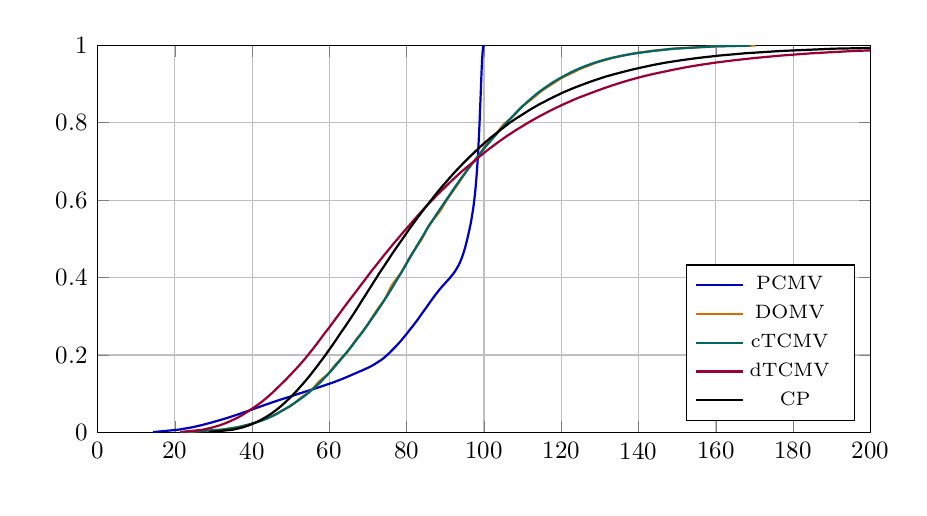
\begin{tikzpicture}
\begin{axis}[width=.94\textwidth,height=6.5cm,xmin=0,xmax=200,ymin=0,ymax=1,xlabel={終端富（年間拠出額単位）},ylabel={累積確率},grid=major,legend style={font=\scriptsize,at={(.98,.03)},anchor=south east},tick label style={font=\small}]
\addplot+[no marks,thick,color=blue!75!black] coordinates {(14.36140,0.00100) (20.83771,0.00700) (24.32792,0.01300) (26.98426,0.01900) (29.24585,0.02500) (31.36509,0.03100) (33.39910,0.03700) (35.23353,0.04300) (37.02775,0.04900) (38.75633,0.05500) (40.44452,0.06100) (42.15555,0.06700) (43.86080,0.07300) (45.60421,0.07900) (47.42656,0.08500) (49.32568,0.09100) (51.14111,0.09700) (52.99687,0.10300) (54.87784,0.10900) (56.75240,0.11500) (58.54717,0.12100) (60.36719,0.12700) (61.97653,0.13300) (63.51198,0.13900) (64.95596,0.14500) (66.32853,0.15100) (67.71761,0.15700) (69.09623,0.16300) (70.40847,0.16900) (71.49179,0.17500) (72.45401,0.18100) (73.37188,0.18700) (74.15940,0.19300) (74.84562,0.19900) (75.49679,0.20500) (76.08134,0.21100) (76.68602,0.21700) (77.26491,0.22300) (77.81512,0.22900) (78.36321,0.23500) (78.86394,0.24100) (79.35985,0.24700) (79.85885,0.25300) (80.34087,0.25900) (80.78920,0.26500) (81.28366,0.27100) (81.75212,0.27700) (82.20932,0.28300) (82.66572,0.28900) (83.10766,0.29500) (83.52570,0.30100) (83.94636,0.30700) (84.36785,0.31300) (84.81191,0.31900) (85.23085,0.32500) (85.65966,0.33100) (86.08495,0.33700) (86.50925,0.34300) (86.96130,0.34900) (87.40439,0.35500) (87.86970,0.36100) (88.34014,0.36700) (88.84090,0.37300) (89.34347,0.37900) (89.90637,0.38500) (90.45467,0.39100) (91.01116,0.39700) (91.50524,0.40300) (91.99562,0.40900) (92.42386,0.41500) (92.81135,0.42100) (93.16343,0.42700) (93.49237,0.43300) (93.77387,0.43900) (94.02046,0.44500) (94.26179,0.45100) (94.48630,0.45700) (94.68056,0.46300) (94.86882,0.46900) (95.05271,0.47500) (95.21227,0.48100) (95.37699,0.48700) (95.52253,0.49300) (95.66992,0.49900) (95.80908,0.50500) (95.94656,0.51100) (96.08271,0.51700) (96.21117,0.52300) (96.34475,0.52900) (96.46775,0.53500) (96.59051,0.54100) (96.69956,0.54700) (96.80256,0.55300) (96.90215,0.55900) (97.00143,0.56500) (97.10062,0.57100) (97.19435,0.57700) (97.27599,0.58300) (97.35498,0.58900) (97.43035,0.59500) (97.50272,0.60100) (97.57091,0.60700) (97.63771,0.61300) (97.70333,0.61900) (97.76381,0.62500) (97.81827,0.63100) (97.87345,0.63700) (97.92703,0.64300) (97.97853,0.64900) (98.02729,0.65500) (98.07445,0.66100) (98.11932,0.66700) (98.16413,0.67300) (98.20501,0.67900) (98.24761,0.68500) (98.28721,0.69100) (98.32462,0.69700) (98.36208,0.70300) (98.39885,0.70900) (98.43389,0.71500) (98.46686,0.72100) (98.49892,0.72700) (98.53202,0.73300) (98.56404,0.73900) (98.59595,0.74500) (98.62728,0.75100) (98.65905,0.75700) (98.68650,0.76300) (98.71472,0.76900) (98.74287,0.77500) (98.77128,0.78100) (98.79934,0.78700) (98.82673,0.79300) (98.85132,0.79900) (98.87661,0.80500) (98.90219,0.81100) (98.92743,0.81700) (98.95162,0.82300) (98.97487,0.82900) (98.99830,0.83500) (99.02280,0.84100) (99.04639,0.84700) (99.06969,0.85300) (99.09247,0.85900) (99.11572,0.86500) (99.13988,0.87100) (99.16190,0.87700) (99.18447,0.88300) (99.20856,0.88900) (99.23143,0.89500) (99.25461,0.90100) (99.27719,0.90700) (99.30037,0.91300) (99.32481,0.91900) (99.34858,0.92500) (99.37172,0.93100) (99.39700,0.93700) (99.42387,0.94300) (99.45258,0.94900) (99.48193,0.95500) (99.51173,0.96100) (99.54596,0.96700) (99.58147,0.97300) (99.62123,0.97900) (99.66759,0.98500) (99.72653,0.99100) (99.82527,0.99700) (99.89525,0.99900)};\addlegendentry{PCMV保存}
\addplot+[no marks,thick,color=orange!85!black] coordinates {(22.67883,0.00100) (31.83856,0.00700) (35.85196,0.01300) (38.45154,0.01900) (40.72800,0.02500) (42.21265,0.03100) (43.74614,0.03700) (45.31071,0.04300) (46.40781,0.04900) (47.44688,0.05500) (48.60684,0.06100) (49.74601,0.06700) (50.59862,0.07300) (51.39210,0.07900) (52.09076,0.08500) (52.80632,0.09100) (53.68236,0.09700) (54.57233,0.10300) (55.27874,0.10900) (55.88578,0.11500) (56.41144,0.12100) (56.92692,0.12700) (57.48931,0.13300) (58.19078,0.13900) (58.95374,0.14500) (59.63875,0.15100) (60.17302,0.15700) (60.62723,0.16300) (61.08886,0.16900) (61.58475,0.17500) (62.10155,0.18100) (62.68319,0.18700) (63.28425,0.19300) (63.86285,0.19900) (64.41538,0.20500) (64.91449,0.21100) (65.34581,0.21700) (65.74695,0.22300) (66.13057,0.22900) (66.55139,0.23500) (66.99797,0.24100) (67.48143,0.24700) (68.01399,0.25300) (68.53326,0.25900) (69.01099,0.26500) (69.43119,0.27100) (69.81587,0.27700) (70.21060,0.28300) (70.57563,0.28900) (70.93942,0.29500) (71.32600,0.30100) (71.71346,0.30700) (72.10542,0.31300) (72.51161,0.31900) (72.95018,0.32500) (73.40863,0.33100) (73.84421,0.33700) (74.25988,0.34300) (74.61281,0.34900) (74.90689,0.35500) (75.19058,0.36100) (75.47852,0.36700) (75.78185,0.37300) (76.12565,0.37900) (76.50569,0.38500) (76.95741,0.39100) (77.40451,0.39700) (77.86616,0.40300) (78.31108,0.40900) (78.68515,0.41500) (79.02067,0.42100) (79.36643,0.42700) (79.70079,0.43300) (80.04631,0.43900) (80.37094,0.44500) (80.72650,0.45100) (81.07874,0.45700) (81.47484,0.46300) (81.87189,0.46900) (82.26287,0.47500) (82.66291,0.48100) (83.09179,0.48700) (83.50201,0.49300) (83.87921,0.49900) (84.21825,0.50500) (84.52363,0.51100) (84.80934,0.51700) (85.09693,0.52300) (85.40809,0.52900) (85.76299,0.53500) (86.17346,0.54100) (86.63973,0.54700) (87.15566,0.55300) (87.66615,0.55900) (88.13626,0.56500) (88.57499,0.57100) (88.96142,0.57700) (89.31618,0.58300) (89.68336,0.58900) (90.04466,0.59500) (90.41321,0.60100) (90.83874,0.60700) (91.24978,0.61300) (91.66894,0.61900) (92.09660,0.62500) (92.51032,0.63100) (92.94055,0.63700) (93.37005,0.64300) (93.76610,0.64900) (94.16827,0.65500) (94.57141,0.66100) (94.97085,0.66700) (95.34888,0.67300) (95.75704,0.67900) (96.19359,0.68500) (96.67850,0.69100) (97.21165,0.69700) (97.74361,0.70300) (98.23146,0.70900) (98.67131,0.71500) (99.07040,0.72100) (99.41888,0.72700) (99.82268,0.73300) (100.26531,0.73900) (100.76790,0.74500) (101.37013,0.75100) (101.99459,0.75700) (102.58186,0.76300) (103.09832,0.76900) (103.52802,0.77500) (103.95129,0.78100) (104.39082,0.78700) (104.90237,0.79300) (105.48976,0.79900) (106.20857,0.80500) (106.92608,0.81100) (107.55773,0.81700) (108.14586,0.82300) (108.67227,0.82900) (109.23766,0.83500) (109.85000,0.84100) (110.57403,0.84700) (111.33169,0.85300) (112.15527,0.85900) (112.86507,0.86500) (113.57198,0.87100) (114.28130,0.87700) (115.07492,0.88300) (115.95125,0.88900) (116.91264,0.89500) (117.86614,0.90100) (118.77151,0.90700) (119.67612,0.91300) (120.77904,0.91900) (122.07470,0.92500) (123.31568,0.93100) (124.47199,0.93700) (125.93917,0.94300) (127.56437,0.94900) (129.05358,0.95500) (131.06767,0.96100) (133.20659,0.96700) (135.89941,0.97300) (138.82643,0.97900) (143.07574,0.98500) (148.70028,0.99100) (159.89571,0.99700) (170.19351,0.99900)};\addlegendentry{DOMV保存}
\addplot+[no marks,thick,color=teal!80!black] coordinates {(21.37548,0.00100) (32.11850,0.00700) (36.17666,0.01300) (38.69904,0.01900) (40.71615,0.02500) (42.60145,0.03100) (44.14452,0.03700) (45.43076,0.04300) (46.58369,0.04900) (47.57439,0.05500) (48.59884,0.06100) (49.60449,0.06700) (50.52308,0.07300) (51.39736,0.07900) (52.26497,0.08500) (53.12251,0.09100) (53.90476,0.09700) (54.64320,0.10300) (55.36575,0.10900) (56.04560,0.11500) (56.71943,0.12100) (57.35876,0.12700) (57.96901,0.13300) (58.54142,0.13900) (59.12462,0.14500) (59.69099,0.15100) (60.24480,0.15700) (60.78886,0.16300) (61.30781,0.16900) (61.81678,0.17500) (62.33263,0.18100) (62.83427,0.18700) (63.31130,0.19300) (63.79290,0.19900) (64.30632,0.20500) (64.79814,0.21100) (65.29175,0.21700) (65.76256,0.22300) (66.23482,0.22900) (66.69299,0.23500) (67.14061,0.24100) (67.61340,0.24700) (68.08069,0.25300) (68.50241,0.25900) (68.92737,0.26500) (69.35366,0.27100) (69.78878,0.27700) (70.22159,0.28300) (70.63125,0.28900) (71.06104,0.29500) (71.47905,0.30100) (71.90636,0.30700) (72.31763,0.31300) (72.72835,0.31900) (73.13010,0.32500) (73.52810,0.33100) (73.90597,0.33700) (74.30217,0.34300) (74.68703,0.34900) (75.08272,0.35500) (75.45581,0.36100) (75.83149,0.36700) (76.19960,0.37300) (76.56151,0.37900) (76.91415,0.38500) (77.27347,0.39100) (77.64842,0.39700) (78.00619,0.40300) (78.38307,0.40900) (78.74189,0.41500) (79.08673,0.42100) (79.44279,0.42700) (79.79102,0.43300) (80.12908,0.43900) (80.47308,0.44500) (80.82954,0.45100) (81.18187,0.45700) (81.53869,0.46300) (81.88556,0.46900) (82.24111,0.47500) (82.59235,0.48100) (82.95189,0.48700) (83.30684,0.49300) (83.67859,0.49900) (84.03655,0.50500) (84.40287,0.51100) (84.77383,0.51700) (85.14118,0.52300) (85.49789,0.52900) (85.88214,0.53500) (86.27272,0.54100) (86.66829,0.54700) (87.05114,0.55300) (87.43794,0.55900) (87.81701,0.56500) (88.22141,0.57100) (88.63549,0.57700) (89.04890,0.58300) (89.45283,0.58900) (89.85549,0.59500) (90.27849,0.60100) (90.69642,0.60700) (91.10216,0.61300) (91.50805,0.61900) (91.90444,0.62500) (92.32323,0.63100) (92.72966,0.63700) (93.14800,0.64300) (93.56964,0.64900) (93.99512,0.65500) (94.44417,0.66100) (94.89542,0.66700) (95.35462,0.67300) (95.79194,0.67900) (96.24996,0.68500) (96.70346,0.69100) (97.16892,0.69700) (97.61543,0.70300) (98.10227,0.70900) (98.58000,0.71500) (99.05898,0.72100) (99.53971,0.72700) (100.03129,0.73300) (100.51560,0.73900) (101.01945,0.74500) (101.53241,0.75100) (102.03128,0.75700) (102.56754,0.76300) (103.08209,0.76900) (103.60670,0.77500) (104.13907,0.78100) (104.69368,0.78700) (105.26353,0.79300) (105.79955,0.79900) (106.33362,0.80500) (106.88712,0.81100) (107.46357,0.81700) (108.03400,0.82300) (108.64339,0.82900) (109.22678,0.83500) (109.83142,0.84100) (110.46721,0.84700) (111.12521,0.85300) (111.80642,0.85900) (112.49993,0.86500) (113.24313,0.87100) (113.96494,0.87700) (114.77842,0.88300) (115.60498,0.88900) (116.46501,0.89500) (117.35367,0.90100) (118.33115,0.90700) (119.33274,0.91300) (120.43378,0.91900) (121.57152,0.92500) (122.73921,0.93100) (124.03239,0.93700) (125.42341,0.94300) (126.99229,0.94900) (128.71744,0.95500) (130.69872,0.96100) (132.94755,0.96700) (135.74371,0.97300) (139.24441,0.97900) (143.72609,0.98500) (149.34778,0.99100) (159.89598,0.99700) (168.90225,0.99900)};\addlegendentry{cTCMV保存}
\addplot+[no marks,thick,color=purple!80!black] coordinates {(21.48290,0.00100) (27.22539,0.00700) (29.76650,0.01300) (31.79039,0.01900) (33.36868,0.02500) (34.74341,0.03100) (35.99686,0.03700) (37.12332,0.04300) (38.08704,0.04900) (39.04562,0.05500) (39.90473,0.06100) (40.82844,0.06700) (41.67899,0.07300) (42.49613,0.07900) (43.22542,0.08500) (43.93779,0.09100) (44.62272,0.09700) (45.29773,0.10300) (45.91455,0.10900) (46.53399,0.11500) (47.15398,0.12100) (47.76263,0.12700) (48.40792,0.13300) (48.98281,0.13900) (49.53274,0.14500) (50.13921,0.15100) (50.69556,0.15700) (51.24757,0.16300) (51.80093,0.16900) (52.34823,0.17500) (52.87532,0.18100) (53.40171,0.18700) (53.89649,0.19300) (54.41090,0.19900) (54.87651,0.20500) (55.35980,0.21100) (55.84352,0.21700) (56.29619,0.22300) (56.77495,0.22900) (57.22174,0.23500) (57.66323,0.24100) (58.09890,0.24700) (58.55318,0.25300) (59.00885,0.25900) (59.48414,0.26500) (59.95672,0.27100) (60.39369,0.27700) (60.83926,0.28300) (61.28396,0.28900) (61.72007,0.29500) (62.17042,0.30100) (62.61382,0.30700) (63.04528,0.31300) (63.48459,0.31900) (63.93525,0.32500) (64.38600,0.33100) (64.83293,0.33700) (65.28494,0.34300) (65.75609,0.34900) (66.21923,0.35500) (66.66960,0.36100) (67.13914,0.36700) (67.58722,0.37300) (68.03882,0.37900) (68.48892,0.38500) (68.95054,0.39100) (69.40732,0.39700) (69.86688,0.40300) (70.31045,0.40900) (70.74946,0.41500) (71.22343,0.42100) (71.71557,0.42700) (72.19701,0.43300) (72.67872,0.43900) (73.13945,0.44500) (73.61822,0.45100) (74.10320,0.45700) (74.58605,0.46300) (75.08088,0.46900) (75.57108,0.47500) (76.06528,0.48100) (76.55526,0.48700) (77.06534,0.49300) (77.60503,0.49900) (78.09557,0.50500) (78.59871,0.51100) (79.11407,0.51700) (79.65201,0.52300) (80.16156,0.52900) (80.68673,0.53500) (81.21428,0.54100) (81.72682,0.54700) (82.26115,0.55300) (82.79258,0.55900) (83.35039,0.56500) (83.86923,0.57100) (84.40558,0.57700) (84.99408,0.58300) (85.53140,0.58900) (86.10277,0.59500) (86.68823,0.60100) (87.27565,0.60700) (87.87123,0.61300) (88.47948,0.61900) (89.07314,0.62500) (89.69165,0.63100) (90.31316,0.63700) (90.90517,0.64300) (91.53132,0.64900) (92.17805,0.65500) (92.82705,0.66100) (93.47934,0.66700) (94.13726,0.67300) (94.85189,0.67900) (95.56324,0.68500) (96.31332,0.69100) (97.00149,0.69700) (97.73199,0.70300) (98.46056,0.70900) (99.16475,0.71500) (99.89744,0.72100) (100.65580,0.72700) (101.43431,0.73300) (102.24307,0.73900) (103.04383,0.74500) (103.88484,0.75100) (104.73206,0.75700) (105.57536,0.76300) (106.46958,0.76900) (107.41228,0.77500) (108.31547,0.78100) (109.31014,0.78700) (110.28268,0.79300) (111.27340,0.79900) (112.32143,0.80500) (113.39849,0.81100) (114.48309,0.81700) (115.61687,0.82300) (116.77678,0.82900) (117.94184,0.83500) (119.21315,0.84100) (120.49516,0.84700) (121.85629,0.85300) (123.20238,0.85900) (124.63477,0.86500) (126.24236,0.87100) (127.81800,0.87700) (129.40818,0.88300) (131.10505,0.88900) (132.84756,0.89500) (134.68325,0.90100) (136.64595,0.90700) (138.74428,0.91300) (141.01321,0.91900) (143.48472,0.92500) (146.30974,0.93100) (149.16200,0.93700) (152.24767,0.94300) (155.84634,0.94900) (159.89755,0.95500) (164.66439,0.96100) (170.14544,0.96700) (176.59614,0.97300) (184.62902,0.97900) (195.58764,0.98500) (212.68976,0.99100) (252.39064,0.99700) (299.43421,0.99900)};\addlegendentry{dTCMV保存}
\addplot+[no marks,thick,color=black] coordinates {(28.78762,0.00100) (34.91494,0.00700) (37.53254,0.01300) (39.30274,0.01900) (40.77758,0.02500) (42.02765,0.03100) (43.10579,0.03700) (44.12039,0.04300) (45.01688,0.04900) (45.82625,0.05500) (46.61454,0.06100) (47.34515,0.06700) (48.03255,0.07300) (48.69862,0.07900) (49.31868,0.08500) (49.95499,0.09100) (50.56407,0.09700) (51.12355,0.10300) (51.67108,0.10900) (52.19972,0.11500) (52.73405,0.12100) (53.26496,0.12700) (53.79137,0.13300) (54.29951,0.13900) (54.78772,0.14500) (55.26976,0.15100) (55.72910,0.15700) (56.19821,0.16300) (56.66497,0.16900) (57.11612,0.17500) (57.55829,0.18100) (58.02623,0.18700) (58.47289,0.19300) (58.91321,0.19900) (59.33116,0.20500) (59.76001,0.21100) (60.18437,0.21700) (60.61264,0.22300) (61.02849,0.22900) (61.44274,0.23500) (61.85736,0.24100) (62.25753,0.24700) (62.64252,0.25300) (63.04764,0.25900) (63.48006,0.26500) (63.90515,0.27100) (64.31544,0.27700) (64.72389,0.28300) (65.12599,0.28900) (65.52854,0.29500) (65.90975,0.30100) (66.31507,0.30700) (66.69487,0.31300) (67.07969,0.31900) (67.47093,0.32500) (67.84133,0.33100) (68.20780,0.33700) (68.58895,0.34300) (68.97111,0.34900) (69.36649,0.35500) (69.73723,0.36100) (70.11770,0.36700) (70.50761,0.37300) (70.88893,0.37900) (71.25237,0.38500) (71.63631,0.39100) (72.02385,0.39700) (72.40162,0.40300) (72.77097,0.40900) (73.18004,0.41500) (73.56857,0.42100) (73.97361,0.42700) (74.36463,0.43300) (74.76895,0.43900) (75.17415,0.44500) (75.56441,0.45100) (75.96461,0.45700) (76.36339,0.46300) (76.76836,0.46900) (77.18734,0.47500) (77.60314,0.48100) (78.02439,0.48700) (78.45206,0.49300) (78.86939,0.49900) (79.28197,0.50500) (79.69965,0.51100) (80.12278,0.51700) (80.52634,0.52300) (80.95297,0.52900) (81.39092,0.53500) (81.83057,0.54100) (82.26860,0.54700) (82.69454,0.55300) (83.14176,0.55900) (83.59939,0.56500) (84.05267,0.57100) (84.52772,0.57700) (84.97722,0.58300) (85.44950,0.58900) (85.93229,0.59500) (86.41004,0.60100) (86.88953,0.60700) (87.36068,0.61300) (87.84597,0.61900) (88.33598,0.62500) (88.82146,0.63100) (89.34839,0.63700) (89.87846,0.64300) (90.38905,0.64900) (90.89862,0.65500) (91.44222,0.66100) (91.97938,0.66700) (92.50906,0.67300) (93.08099,0.67900) (93.65687,0.68500) (94.24026,0.69100) (94.82883,0.69700) (95.43337,0.70300) (96.03589,0.70900) (96.64015,0.71500) (97.28926,0.72100) (97.90435,0.72700) (98.55584,0.73300) (99.20099,0.73900) (99.85495,0.74500) (100.53847,0.75100) (101.24069,0.75700) (101.96838,0.76300) (102.72516,0.76900) (103.50357,0.77500) (104.21877,0.78100) (105.01145,0.78700) (105.80266,0.79300) (106.55528,0.79900) (107.43940,0.80500) (108.34994,0.81100) (109.31227,0.81700) (110.26571,0.82300) (111.20209,0.82900) (112.16963,0.83500) (113.21599,0.84100) (114.25844,0.84700) (115.42316,0.85300) (116.58738,0.85900) (117.76234,0.86500) (119.01639,0.87100) (120.26452,0.87700) (121.65769,0.88300) (123.09366,0.88900) (124.63873,0.89500) (126.25231,0.90100) (127.88340,0.90700) (129.67211,0.91300) (131.53017,0.91900) (133.68799,0.92500) (135.98520,0.93100) (138.37885,0.93700) (141.01978,0.94300) (143.82042,0.94900) (147.01971,0.95500) (150.92447,0.96100) (155.35661,0.96700) (160.65939,0.97300) (167.43155,0.97900) (176.75134,0.98500) (190.61167,0.99100) (221.52242,0.99700) (251.38090,0.99900)};\addlegendentry{CP}
\end{axis}\end{tikzpicture}
\caption{保存方策とCPの経験終端CDF．20万経路から生成．}\label{fig:cdf}
\end{figure}
図\ref{fig:cdf}は20万経路の経験分位点から描いた終端CDFである．曲線は保存方策の性能を示し，解析的な最適分布ではない．正規Euler再評価で300超を経験した割合はdTCMV保存方策で約0.137\%，CPで約0.030\%であった．小さい確率でも上位裾への寄与は無視できないため，dTCMVのUCVaRを高精度に確定したとは扱わない．全基準経路で負残高の切上げは発生しなかったが，発生確率が理論的にゼロであることは意味しない．

\subsection{同じ係数・固定ターゲットでのクリップ比較}
\begin{table}[htbp]\centering\small
\caption{クリップと保存方策の成果差：同一入力による診断}\label{tab:clip}
\begin{tabular}{lrrrr}
\toprule
解概念 & $G_{\mathrm{MAE}}$ & 平均差 & 平均差の95\%区間 & LCVaR差 \\ \midrule
PCMV & 0.030 & 1.654 & [1.634, 1.673] & -1.405 \\
DOMV & 0.086 & 3.748 & [3.715, 3.780] & -3.294 \\
cTCMV & 0.018 & -1.990 & [-2.005, -1.975] & 0.091 \\
dTCMV & 0.147 & 4.473 & [4.437, 4.508] & 0.952 \\
\bottomrule\end{tabular}
\par\vspace{3pt}\begin{minipage}{0.97\textwidth}\footnotesize 差はクリップ－保存方策．PCMVは固定ターゲット比較．dTCMVクリップには修正後の無制約係数を使用する．LCVaR差の信頼区間は推定していない．\end{minipage}
\end{table}
表\ref{tab:clip}の差は「クリップ－保存方策」である．各方策の平均差の信頼区間には，共通乱数による経路ごとの差の標準誤差を用いる．これにより，独立の標本同士を比較するより差を精密に推定できる．ただし，信頼区間は固定された方策・モデルのサンプリング誤差だけを表す．

PCMVとDOMVでは，この設定のクリップは平均を高める一方，LCVaRを下げる．cTCMVのクリップは平均を約1.99下げ，LCVaR差は約0.09にとどまる．平均配分差の小ささだけから，成果の近似が十分とは結論できない．

修正したdTCMVクリップでは，保存方策に比べ平均が約4.47高く，LCVaRも約0.95高い．したがって，従来の診断値を根拠に「dTCMVのクリップは下方裾を悪化させる」と一般化することはできない．この変化には無制約係数，評価方法および比較設定の修正が含まれ，符号変更だけの因果効果を識別したものでもない．保存方策を真の均衡とみなして，クリップが均衡を経済的に優越すると結論することもできない．

\begin{figure}[htbp]\centering
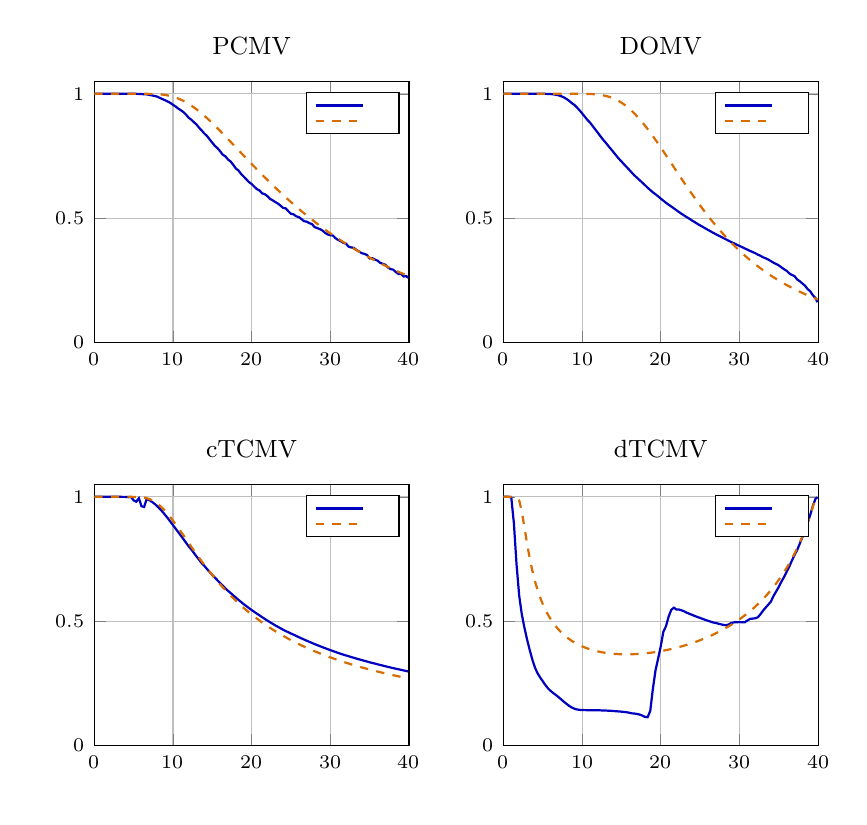
\begin{tikzpicture}
\begin{groupplot}[group style={group size=2 by 2,horizontal sep=1.2cm,vertical sep=1.8cm},width=.46\textwidth,height=4.9cm,xmin=0,xmax=40,ymin=0,ymax=1.05,xlabel={経過年},ylabel={平均リスク資産比率},grid=major,tick label style={font=\scriptsize},label style={font=\scriptsize},title style={font=\small},legend style={font=\tiny,at={(.97,.96)},anchor=north east}]
\nextgroupplot[title={PCMV}]
\addplot+[no marks,thick,color=blue!75!black] coordinates {(0.00000,1.00000) (0.33333,1.00000) (0.66667,1.00000) (1.00000,1.00000) (1.33333,1.00000) (1.66667,1.00000) (2.00000,1.00000) (2.33333,1.00000) (2.66667,1.00000) (3.00000,1.00000) (3.33333,1.00000) (3.66667,1.00000) (4.00000,1.00000) (4.33333,1.00000) (4.66667,1.00000) (5.00000,0.99997) (5.33333,0.99988) (5.66667,0.99965) (6.00000,0.99911) (6.33333,0.99821) (6.66667,0.99770) (7.00000,0.99587) (7.33333,0.99370) (7.66667,0.99138) (8.00000,0.98877) (8.33333,0.98359) (8.66667,0.97883) (9.00000,0.97414) (9.33333,0.96902) (9.66667,0.96356) (10.00000,0.95580) (10.33333,0.94924) (10.66667,0.94079) (11.00000,0.93398) (11.33333,0.92669) (11.66667,0.91630) (12.00000,0.90362) (12.33333,0.89615) (12.66667,0.88586) (13.00000,0.87653) (13.33333,0.86343) (13.66667,0.85226) (14.00000,0.84034) (14.33333,0.83031) (14.66667,0.81677) (15.00000,0.80338) (15.33333,0.79059) (15.66667,0.78155) (16.00000,0.76908) (16.33333,0.75537) (16.66667,0.74866) (17.00000,0.73597) (17.33333,0.72798) (17.66667,0.71461) (18.00000,0.69978) (18.33333,0.69180) (18.66667,0.67788) (19.00000,0.66744) (19.33333,0.65602) (19.66667,0.64533) (20.00000,0.63758) (20.33333,0.62722) (20.66667,0.61700) (21.00000,0.61191) (21.33333,0.60009) (21.66667,0.59657) (22.00000,0.58927) (22.33333,0.57818) (22.66667,0.57221) (23.00000,0.56523) (23.33333,0.55915) (23.66667,0.55102) (24.00000,0.54153) (24.33333,0.53974) (24.66667,0.52840) (25.00000,0.51804) (25.33333,0.51569) (25.66667,0.50774) (26.00000,0.50462) (26.33333,0.49681) (26.66667,0.48807) (27.00000,0.48648) (27.33333,0.48032) (27.66667,0.47674) (28.00000,0.46461) (28.33333,0.46063) (28.66667,0.45642) (29.00000,0.45079) (29.33333,0.44135) (29.66667,0.43476) (30.00000,0.43194) (30.33333,0.43059) (30.66667,0.41963) (31.00000,0.41281) (31.33333,0.40782) (31.66667,0.40089) (32.00000,0.39796) (32.33333,0.38565) (32.66667,0.38268) (33.00000,0.38077) (33.33333,0.37218) (33.66667,0.36608) (34.00000,0.35978) (34.33333,0.35693) (34.66667,0.35241) (35.00000,0.33861) (35.33333,0.33956) (35.66667,0.33421) (36.00000,0.32985) (36.33333,0.32092) (36.66667,0.31713) (37.00000,0.31307) (37.33333,0.30208) (37.66667,0.29560) (38.00000,0.29352) (38.33333,0.28363) (38.66667,0.27627) (39.00000,0.27577) (39.33333,0.26602) (39.66667,0.26728) (39.91667,0.26062)};\addlegendentry{保存方策}
\addplot+[no marks,thick,dashed,color=orange!85!black] coordinates {(0.00000,1.00000) (0.33333,1.00000) (0.66667,1.00000) (1.00000,1.00000) (1.33333,1.00000) (1.66667,1.00000) (2.00000,1.00000) (2.33333,1.00000) (2.66667,1.00000) (3.00000,1.00000) (3.33333,1.00000) (3.66667,1.00000) (4.00000,1.00000) (4.33333,1.00000) (4.66667,1.00000) (5.00000,1.00000) (5.33333,1.00000) (5.66667,0.99999) (6.00000,0.99999) (6.33333,0.99996) (6.66667,0.99991) (7.00000,0.99980) (7.33333,0.99960) (7.66667,0.99931) (8.00000,0.99885) (8.33333,0.99802) (8.66667,0.99693) (9.00000,0.99550) (9.33333,0.99361) (9.66667,0.99126) (10.00000,0.98820) (10.33333,0.98486) (10.66667,0.98099) (11.00000,0.97641) (11.33333,0.97140) (11.66667,0.96558) (12.00000,0.95933) (12.33333,0.95268) (12.66667,0.94526) (13.00000,0.93764) (13.33333,0.92930) (13.66667,0.92063) (14.00000,0.91146) (14.33333,0.90209) (14.66667,0.89243) (15.00000,0.88232) (15.33333,0.87205) (15.66667,0.86157) (16.00000,0.85085) (16.33333,0.84009) (16.66667,0.82922) (17.00000,0.81796) (17.33333,0.80707) (17.66667,0.79586) (18.00000,0.78470) (18.33333,0.77357) (18.66667,0.76241) (19.00000,0.75135) (19.33333,0.74036) (19.66667,0.72938) (20.00000,0.71840) (20.33333,0.70748) (20.66667,0.69656) (21.00000,0.68580) (21.33333,0.67499) (21.66667,0.66456) (22.00000,0.65419) (22.33333,0.64362) (22.66667,0.63351) (23.00000,0.62336) (23.33333,0.61342) (23.66667,0.60368) (24.00000,0.59404) (24.33333,0.58414) (24.66667,0.57442) (25.00000,0.56511) (25.33333,0.55598) (25.66667,0.54686) (26.00000,0.53783) (26.33333,0.52866) (26.66667,0.51994) (27.00000,0.51138) (27.33333,0.50293) (27.66667,0.49466) (28.00000,0.48634) (28.33333,0.47790) (28.66667,0.47001) (29.00000,0.46210) (29.33333,0.45427) (29.66667,0.44653) (30.00000,0.43931) (30.33333,0.43221) (30.66667,0.42487) (31.00000,0.41794) (31.33333,0.41088) (31.66667,0.40409) (32.00000,0.39757) (32.33333,0.39100) (32.66667,0.38450) (33.00000,0.37793) (33.33333,0.37167) (33.66667,0.36558) (34.00000,0.35945) (34.33333,0.35364) (34.66667,0.34775) (35.00000,0.34190) (35.33333,0.33610) (35.66667,0.33052) (36.00000,0.32511) (36.33333,0.31976) (36.66667,0.31431) (37.00000,0.30916) (37.33333,0.30396) (37.66667,0.29889) (38.00000,0.29395) (38.33333,0.28931) (38.66667,0.28461) (39.00000,0.28017) (39.33333,0.27567) (39.66667,0.27124) (39.91667,0.26802)};\addlegendentry{クリップ}
\nextgroupplot[title={DOMV}]
\addplot+[no marks,thick,color=blue!75!black] coordinates {(0.00000,1.00000) (0.33333,1.00000) (0.66667,1.00000) (1.00000,1.00000) (1.33333,1.00000) (1.66667,1.00000) (2.00000,1.00000) (2.33333,1.00000) (2.66667,1.00000) (3.00000,1.00000) (3.33333,1.00000) (3.66667,1.00000) (4.00000,1.00000) (4.33333,1.00000) (4.66667,0.99999) (5.00000,0.99996) (5.33333,0.99988) (5.66667,0.99966) (6.00000,0.99911) (6.33333,0.99806) (6.66667,0.99627) (7.00000,0.99414) (7.33333,0.99066) (7.66667,0.98591) (8.00000,0.97978) (8.33333,0.97225) (8.66667,0.96330) (9.00000,0.95589) (9.33333,0.94544) (9.66667,0.93397) (10.00000,0.92165) (10.33333,0.90867) (10.66667,0.89547) (11.00000,0.88456) (11.33333,0.87104) (11.66667,0.85723) (12.00000,0.84353) (12.33333,0.82938) (12.66667,0.81578) (13.00000,0.80380) (13.33333,0.79043) (13.66667,0.77808) (14.00000,0.76513) (14.33333,0.75206) (14.66667,0.73926) (15.00000,0.72831) (15.33333,0.71660) (15.66667,0.70574) (16.00000,0.69431) (16.33333,0.68272) (16.66667,0.67171) (17.00000,0.66220) (17.33333,0.65250) (17.66667,0.64281) (18.00000,0.63271) (18.33333,0.62256) (18.66667,0.61322) (19.00000,0.60426) (19.33333,0.59624) (19.66667,0.58793) (20.00000,0.57891) (20.33333,0.57056) (20.66667,0.56208) (21.00000,0.55438) (21.33333,0.54733) (21.66667,0.53969) (22.00000,0.53226) (22.33333,0.52451) (22.66667,0.51732) (23.00000,0.51057) (23.33333,0.50390) (23.66667,0.49733) (24.00000,0.49047) (24.33333,0.48401) (24.66667,0.47735) (25.00000,0.47125) (25.33333,0.46532) (25.66667,0.45930) (26.00000,0.45319) (26.33333,0.44747) (26.66667,0.44155) (27.00000,0.43589) (27.33333,0.43048) (27.66667,0.42522) (28.00000,0.41969) (28.33333,0.41448) (28.66667,0.40903) (29.00000,0.40378) (29.33333,0.39875) (29.66667,0.39365) (30.00000,0.38884) (30.33333,0.38416) (30.66667,0.37897) (31.00000,0.37396) (31.33333,0.36879) (31.66667,0.36453) (32.00000,0.35961) (32.33333,0.35409) (32.66667,0.34921) (33.00000,0.34318) (33.33333,0.33909) (33.66667,0.33383) (34.00000,0.32782) (34.33333,0.32141) (34.66667,0.31614) (35.00000,0.31056) (35.33333,0.30277) (35.66667,0.29515) (36.00000,0.28874) (36.33333,0.27866) (36.66667,0.27207) (37.00000,0.26753) (37.33333,0.25422) (37.66667,0.24697) (38.00000,0.23796) (38.33333,0.22908) (38.66667,0.21553) (39.00000,0.20635) (39.33333,0.19068) (39.66667,0.17940) (39.91667,0.16239)};\addlegendentry{保存方策}
\addplot+[no marks,thick,dashed,color=orange!85!black] coordinates {(0.00000,1.00000) (0.33333,1.00000) (0.66667,1.00000) (1.00000,1.00000) (1.33333,1.00000) (1.66667,1.00000) (2.00000,1.00000) (2.33333,1.00000) (2.66667,1.00000) (3.00000,1.00000) (3.33333,1.00000) (3.66667,1.00000) (4.00000,1.00000) (4.33333,1.00000) (4.66667,1.00000) (5.00000,1.00000) (5.33333,1.00000) (5.66667,1.00000) (6.00000,1.00000) (6.33333,1.00000) (6.66667,1.00000) (7.00000,1.00000) (7.33333,1.00000) (7.66667,1.00000) (8.00000,1.00000) (8.33333,1.00000) (8.66667,0.99999) (9.00000,0.99998) (9.33333,0.99996) (9.66667,0.99991) (10.00000,0.99984) (10.33333,0.99972) (10.66667,0.99952) (11.00000,0.99919) (11.33333,0.99871) (11.66667,0.99799) (12.00000,0.99694) (12.33333,0.99562) (12.66667,0.99383) (13.00000,0.99161) (13.33333,0.98886) (13.66667,0.98541) (14.00000,0.98136) (14.33333,0.97653) (14.66667,0.97095) (15.00000,0.96449) (15.33333,0.95734) (15.66667,0.94931) (16.00000,0.94045) (16.33333,0.93081) (16.66667,0.92042) (17.00000,0.90917) (17.33333,0.89747) (17.66667,0.88498) (18.00000,0.87196) (18.33333,0.85841) (18.66667,0.84432) (19.00000,0.82989) (19.33333,0.81508) (19.66667,0.79994) (20.00000,0.78448) (20.33333,0.76887) (20.66667,0.75304) (21.00000,0.73722) (21.33333,0.72116) (21.66667,0.70516) (22.00000,0.68923) (22.33333,0.67317) (22.66667,0.65749) (23.00000,0.64185) (23.33333,0.62634) (23.66667,0.61100) (24.00000,0.59580) (24.33333,0.58082) (24.66667,0.56601) (25.00000,0.55151) (25.33333,0.53728) (25.66667,0.52331) (26.00000,0.50971) (26.33333,0.49630) (26.66667,0.48324) (27.00000,0.47058) (27.33333,0.45821) (27.66667,0.44617) (28.00000,0.43438) (28.33333,0.42284) (28.66667,0.41176) (29.00000,0.40074) (29.33333,0.39007) (29.66667,0.37963) (30.00000,0.36963) (30.33333,0.35992) (30.66667,0.35046) (31.00000,0.34131) (31.33333,0.33235) (31.66667,0.32365) (32.00000,0.31526) (32.33333,0.30713) (32.66667,0.29922) (33.00000,0.29149) (33.33333,0.28400) (33.66667,0.27677) (34.00000,0.26972) (34.33333,0.26290) (34.66667,0.25627) (35.00000,0.24983) (35.33333,0.24361) (35.66667,0.23754) (36.00000,0.23166) (36.33333,0.22595) (36.66667,0.22040) (37.00000,0.21504) (37.33333,0.20981) (37.66667,0.20470) (38.00000,0.19978) (38.33333,0.19501) (38.66667,0.19038) (39.00000,0.18588) (39.33333,0.18148) (39.66667,0.17721) (39.91667,0.17410)};\addlegendentry{クリップ}
\nextgroupplot[title={cTCMV}]
\addplot+[no marks,thick,color=blue!75!black] coordinates {(0.00000,1.00000) (0.33333,1.00000) (0.66667,1.00000) (1.00000,1.00000) (1.33333,1.00000) (1.66667,1.00000) (2.00000,1.00000) (2.33333,1.00000) (2.66667,1.00000) (3.00000,1.00000) (3.33333,0.99998) (3.66667,0.99996) (4.00000,0.99972) (4.33333,0.99866) (4.66667,0.99946) (5.00000,0.98593) (5.33333,0.98076) (5.66667,0.99439) (6.00000,0.96221) (6.33333,0.95934) (6.66667,0.99174) (7.00000,0.98656) (7.33333,0.97997) (7.66667,0.97189) (8.00000,0.96251) (8.33333,0.95183) (8.66667,0.94013) (9.00000,0.92775) (9.33333,0.91439) (9.66667,0.90056) (10.00000,0.88660) (10.33333,0.87251) (10.66667,0.85849) (11.00000,0.84424) (11.33333,0.82993) (11.66667,0.81551) (12.00000,0.80096) (12.33333,0.78875) (12.66667,0.77435) (13.00000,0.76023) (13.33333,0.74672) (13.66667,0.73306) (14.00000,0.72222) (14.33333,0.70978) (14.66667,0.69762) (15.00000,0.68567) (15.33333,0.67554) (15.66667,0.66433) (16.00000,0.65333) (16.33333,0.64241) (16.66667,0.63211) (17.00000,0.62220) (17.33333,0.61345) (17.66667,0.60407) (18.00000,0.59513) (18.33333,0.58593) (18.66667,0.57738) (19.00000,0.56861) (19.33333,0.56084) (19.66667,0.55295) (20.00000,0.54530) (20.33333,0.53791) (20.66667,0.53080) (21.00000,0.52370) (21.33333,0.51655) (21.66667,0.50970) (22.00000,0.50286) (22.33333,0.49633) (22.66667,0.48995) (23.00000,0.48365) (23.33333,0.47771) (23.66667,0.47194) (24.00000,0.46615) (24.33333,0.46046) (24.66667,0.45612) (25.00000,0.45071) (25.33333,0.44619) (25.66667,0.44107) (26.00000,0.43618) (26.33333,0.43132) (26.66667,0.42662) (27.00000,0.42191) (27.33333,0.41733) (27.66667,0.41296) (28.00000,0.40852) (28.33333,0.40424) (28.66667,0.40015) (29.00000,0.39599) (29.33333,0.39197) (29.66667,0.38802) (30.00000,0.38412) (30.33333,0.38042) (30.66667,0.37670) (31.00000,0.37273) (31.33333,0.36915) (31.66667,0.36568) (32.00000,0.36272) (32.33333,0.35947) (32.66667,0.35625) (33.00000,0.35312) (33.33333,0.34997) (33.66667,0.34699) (34.00000,0.34402) (34.33333,0.34114) (34.66667,0.33824) (35.00000,0.33531) (35.33333,0.33259) (35.66667,0.32996) (36.00000,0.32721) (36.33333,0.32452) (36.66667,0.32202) (37.00000,0.31925) (37.33333,0.31673) (37.66667,0.31424) (38.00000,0.31178) (38.33333,0.30940) (38.66667,0.30720) (39.00000,0.30482) (39.33333,0.30244) (39.66667,0.29999) (39.91667,0.29815)};\addlegendentry{保存方策}
\addplot+[no marks,thick,dashed,color=orange!85!black] coordinates {(0.00000,1.00000) (0.33333,1.00000) (0.66667,1.00000) (1.00000,1.00000) (1.33333,1.00000) (1.66667,1.00000) (2.00000,1.00000) (2.33333,1.00000) (2.66667,1.00000) (3.00000,1.00000) (3.33333,1.00000) (3.66667,1.00000) (4.00000,1.00000) (4.33333,1.00000) (4.66667,0.99999) (5.00000,0.99993) (5.33333,0.99976) (5.66667,0.99935) (6.00000,0.99848) (6.33333,0.99701) (6.66667,0.99468) (7.00000,0.99124) (7.33333,0.98661) (7.66667,0.98055) (8.00000,0.97320) (8.33333,0.96447) (8.66667,0.95445) (9.00000,0.94349) (9.33333,0.93122) (9.66667,0.91828) (10.00000,0.90435) (10.33333,0.89009) (10.66667,0.87561) (11.00000,0.86061) (11.33333,0.84547) (11.66667,0.83038) (12.00000,0.81473) (12.33333,0.79953) (12.66667,0.78444) (13.00000,0.76948) (13.33333,0.75489) (13.66667,0.74041) (14.00000,0.72624) (14.33333,0.71249) (14.66667,0.69906) (15.00000,0.68593) (15.33333,0.67304) (15.66667,0.66068) (16.00000,0.64849) (16.33333,0.63661) (16.66667,0.62518) (17.00000,0.61399) (17.33333,0.60325) (17.66667,0.59273) (18.00000,0.58252) (18.33333,0.57260) (18.66667,0.56296) (19.00000,0.55356) (19.33333,0.54446) (19.66667,0.53572) (20.00000,0.52717) (20.33333,0.51890) (20.66667,0.51087) (21.00000,0.50308) (21.33333,0.49541) (21.66667,0.48799) (22.00000,0.48077) (22.33333,0.47368) (22.66667,0.46704) (23.00000,0.46041) (23.33333,0.45391) (23.66667,0.44772) (24.00000,0.44163) (24.33333,0.43573) (24.66667,0.42987) (25.00000,0.42415) (25.33333,0.41868) (25.66667,0.41333) (26.00000,0.40815) (26.33333,0.40309) (26.66667,0.39819) (27.00000,0.39338) (27.33333,0.38871) (27.66667,0.38417) (28.00000,0.37971) (28.33333,0.37531) (28.66667,0.37112) (29.00000,0.36687) (29.33333,0.36281) (29.66667,0.35875) (30.00000,0.35488) (30.33333,0.35113) (30.66667,0.34742) (31.00000,0.34385) (31.33333,0.34029) (31.66667,0.33679) (32.00000,0.33344) (32.33333,0.33017) (32.66667,0.32696) (33.00000,0.32375) (33.33333,0.32063) (33.66667,0.31763) (34.00000,0.31463) (34.33333,0.31173) (34.66667,0.30886) (35.00000,0.30607) (35.33333,0.30334) (35.66667,0.30064) (36.00000,0.29801) (36.33333,0.29547) (36.66667,0.29291) (37.00000,0.29046) (37.33333,0.28801) (37.66667,0.28557) (38.00000,0.28324) (38.33333,0.28098) (38.66667,0.27874) (39.00000,0.27655) (39.33333,0.27436) (39.66667,0.27222) (39.91667,0.27065)};\addlegendentry{クリップ}
\nextgroupplot[title={dTCMV}]
\addplot+[no marks,thick,color=blue!75!black] coordinates {(0.00000,1.00000) (0.33333,1.00000) (0.66667,1.00000) (1.00000,0.99754) (1.33333,0.89245) (1.66667,0.72838) (2.00000,0.60363) (2.33333,0.52838) (2.66667,0.47453) (3.00000,0.42750) (3.33333,0.38569) (3.66667,0.34707) (4.00000,0.31436) (4.33333,0.29119) (4.66667,0.27447) (5.00000,0.25895) (5.33333,0.24369) (5.66667,0.23044) (6.00000,0.22007) (6.33333,0.21173) (6.66667,0.20376) (7.00000,0.19530) (7.33333,0.18632) (7.66667,0.17728) (8.00000,0.16856) (8.33333,0.16053) (8.66667,0.15381) (9.00000,0.14885) (9.33333,0.14573) (9.66667,0.14405) (10.00000,0.14329) (10.33333,0.14298) (10.66667,0.14284) (11.00000,0.14274) (11.33333,0.14262) (11.66667,0.14251) (12.00000,0.14237) (12.33333,0.14202) (12.66667,0.14160) (13.00000,0.14118) (13.33333,0.14073) (13.66667,0.14020) (14.00000,0.13942) (14.33333,0.13857) (14.66667,0.13771) (15.00000,0.13679) (15.33333,0.13576) (15.66667,0.13441) (16.00000,0.13237) (16.33333,0.13006) (16.66667,0.12914) (17.00000,0.12746) (17.33333,0.12491) (17.66667,0.12104) (18.00000,0.11562) (18.33333,0.11457) (18.66667,0.14054) (19.00000,0.22936) (19.33333,0.30273) (19.66667,0.35039) (20.00000,0.39982) (20.33333,0.45873) (20.66667,0.48018) (21.00000,0.51873) (21.33333,0.54604) (21.66667,0.55462) (22.00000,0.54700) (22.33333,0.54707) (22.66667,0.54368) (23.00000,0.53960) (23.33333,0.53405) (23.66667,0.52976) (24.00000,0.52554) (24.33333,0.52114) (24.66667,0.51719) (25.00000,0.51342) (25.33333,0.50969) (25.66667,0.50543) (26.00000,0.50194) (26.33333,0.49848) (26.66667,0.49501) (27.00000,0.49324) (27.33333,0.49029) (27.66667,0.48757) (28.00000,0.48523) (28.33333,0.48357) (28.66667,0.48793) (29.00000,0.49339) (29.33333,0.49565) (29.66667,0.49632) (30.00000,0.49674) (30.33333,0.49616) (30.66667,0.49622) (31.00000,0.50282) (31.33333,0.50943) (31.66667,0.51066) (32.00000,0.51211) (32.33333,0.51592) (32.66667,0.52794) (33.00000,0.54269) (33.33333,0.55497) (33.66667,0.56689) (34.00000,0.57915) (34.33333,0.60170) (34.66667,0.61981) (35.00000,0.63828) (35.33333,0.65897) (35.66667,0.67753) (36.00000,0.69861) (36.33333,0.71916) (36.66667,0.74381) (37.00000,0.76618) (37.33333,0.78562) (37.66667,0.81148) (38.00000,0.83822) (38.33333,0.86351) (38.66667,0.89431) (39.00000,0.92747) (39.33333,0.96353) (39.66667,0.99216) (39.91667,0.99800)};\addlegendentry{保存方策}
\addplot+[no marks,thick,dashed,color=orange!85!black] coordinates {(0.00000,1.00000) (0.33333,1.00000) (0.66667,1.00000) (1.00000,1.00000) (1.33333,1.00000) (1.66667,0.99927) (2.00000,0.98582) (2.33333,0.94195) (2.66667,0.87821) (3.00000,0.81283) (3.33333,0.75453) (3.66667,0.70432) (4.00000,0.66206) (4.33333,0.62621) (4.66667,0.59551) (5.00000,0.56915) (5.33333,0.54626) (5.66667,0.52618) (6.00000,0.50857) (6.33333,0.49298) (6.66667,0.47917) (7.00000,0.46687) (7.33333,0.45581) (7.66667,0.44590) (8.00000,0.43702) (8.33333,0.42899) (8.66667,0.42180) (9.00000,0.41529) (9.33333,0.40941) (9.66667,0.40403) (10.00000,0.39921) (10.33333,0.39486) (10.66667,0.39100) (11.00000,0.38743) (11.33333,0.38427) (11.66667,0.38147) (12.00000,0.37889) (12.33333,0.37668) (12.66667,0.37469) (13.00000,0.37298) (13.33333,0.37157) (13.66667,0.37033) (14.00000,0.36931) (14.33333,0.36852) (14.66667,0.36791) (15.00000,0.36747) (15.33333,0.36722) (15.66667,0.36717) (16.00000,0.36726) (16.33333,0.36750) (16.66667,0.36792) (17.00000,0.36847) (17.33333,0.36920) (17.66667,0.37006) (18.00000,0.37105) (18.33333,0.37218) (18.66667,0.37345) (19.00000,0.37485) (19.33333,0.37639) (19.66667,0.37809) (20.00000,0.37991) (20.33333,0.38187) (20.66667,0.38396) (21.00000,0.38620) (21.33333,0.38854) (21.66667,0.39103) (22.00000,0.39366) (22.33333,0.39642) (22.66667,0.39936) (23.00000,0.40241) (23.33333,0.40560) (23.66667,0.40898) (24.00000,0.41249) (24.33333,0.41615) (24.66667,0.41996) (25.00000,0.42393) (25.33333,0.42809) (25.66667,0.43241) (26.00000,0.43693) (26.33333,0.44162) (26.66667,0.44651) (27.00000,0.45161) (27.33333,0.45691) (27.66667,0.46243) (28.00000,0.46816) (28.33333,0.47412) (28.66667,0.48034) (29.00000,0.48678) (29.33333,0.49350) (29.66667,0.50048) (30.00000,0.50778) (30.33333,0.51541) (30.66667,0.52333) (31.00000,0.53161) (31.33333,0.54023) (31.66667,0.54922) (32.00000,0.55864) (32.33333,0.56847) (32.66667,0.57876) (33.00000,0.58951) (33.33333,0.60078) (33.66667,0.61261) (34.00000,0.62500) (34.33333,0.63803) (34.66667,0.65173) (35.00000,0.66616) (35.33333,0.68136) (35.66667,0.69742) (36.00000,0.71439) (36.33333,0.73237) (36.66667,0.75143) (37.00000,0.77169) (37.33333,0.79325) (37.66667,0.81626) (38.00000,0.84087) (38.33333,0.86726) (38.66667,0.89564) (39.00000,0.92623) (39.33333,0.95934) (39.66667,0.99525) (39.91667,1.00000)};\addlegendentry{クリップ}
\end{groupplot}\end{tikzpicture}
\caption{同一入力による保存方策とクリップの平均配分比較．各方策自身の分布で平均．}\label{fig:glide}
\end{figure}
図\ref{fig:glide}は各方策自身の残高分布で平均した比率であり，一人の加入者の実現経路でも年齢だけの配分規則でもない．すべての曲線は最終意思決定時点$T-\Delta t$まで描き，未定義の終端制御をゼロで補完しない．

\subsection{補足監査と結果の位置づけ}
\begin{table}[htbp]\centering\small
\caption{格子配分のない三つの評価方法による標準偏差}\label{tab:robust}
\begin{tabular}{lrrr}
\toprule
方策 & 正規Euler & GH抽出Euler & 月次買持ち \\ \midrule
PCMV保存 & 19.77 & 19.76 & 19.73 \\
DOMV保存 & 24.71 & 24.67 & 24.86 \\
cTCMV保存 & 24.60 & 24.58 & 24.77 \\
dTCMV保存 & 38.20 & 38.27 & 38.47 \\
CP & 31.75 & 31.73 & 32.08 \\
\bottomrule\end{tabular}
\par\vspace{3pt}\begin{minipage}{0.97\textwidth}\footnotesize 正規Eulerは20万経路，他は各10万経路．すべて同じ保存方策・CP比率．月次買持ちは期末拠出を伴う別の運用仕様．\end{minipage}
\end{table}
表\ref{tab:robust}のGH抽出でも標準偏差は正規Eulerの再評価に近い．これは，参照格子との差をGH次数だけに帰する説明を支持しない．月次買持ちでも同様の水準だが，この近さをすべてのパラメータに一般化しない．ここでは各評価方法の乱数系列は独立比較として扱い，方法間の有意差検定は行っていない．

さらに，保存方策の継続モーメントを共通の上端集約モデルで計算し，命題\ref{prop:breakpoints}による一段階逸脱を調べた．到達確率と時点で平均した目的差はcTCMVで約$3.10\times10^{-4}$，dTCMVで約$1.53\times10^{-3}$であった．全格子上の最大差はそれぞれ7.24，5.02で，上端付近に現れた．全格子最大値と到達確率加重値は意味が異なる．また，参照後退ソルバーの上端線形外挿を本監査では集約へ統一しているため，これは元コードの同一目的上の残差をそのまま測った値ではない．境界仕様の相違を含めて，保存方策を\emph{共通の行確率遷移モデルの厳密な一段階均衡}と扱えないことを確認する監査である．

\section{共通期待終価への再最適化と再較正}
\label{sec:equalmean}
\subsection{比較を成立させる計算仕様}
前節までの保存方策監査を受け，四つの意思決定原理に従って方策を新たに計算し，共通期待終価$m_*=84.78$へ再較正した．以下は保存方策の係数だけを事後的に置換した結果ではない．PCMVでは固定ターゲット問題を解き直し，cTCMV・dTCMVでは継続モーメントを後退更新する均衡計算を各係数について実行した．DOMVでは固定ターゲット方策群を再計算し，各時点・各残高で埋め込みスコアを比較して第一期の投資額を選び直した．

全戦略に月次Euler遷移，$[0,600]$の残高範囲，非負の線形確率配分，上端集約を共通に適用する．基準計算は残高刻み0.2，65個の投資比率，5点GH，精緻化計算は残高刻み0.1，129個の投資比率，7点GHである．各格子状態では投資比率$\{j/128:j=0,\ldots,128\}$をすべて比較する．この全数探索は\emph{有限制御集合上}の大域探索であり，連続制御全体に対する大域最適性の証明とは区別する．

較正用評価では，投資額の補間と残高の遷移を分け，より細かい残高刻み0.025と31点GHを用いる．初期残高は正確に$x_0=1/12$から遷移させる．さらに独立した正規乱数を用い，残高を格子へ配分せず，上端で打ち切らないシミュレーションで評価する．較正値そのものと，独立標本で観測される平均の違いを表中に分けて示す．

係数探索では各試行で方策を再計算し，目標平均との差が最も小さい試行を保存する．有限制御集合の均衡選択は係数に対して不連続となり得るため，二分探索の使用を単調性・解の存在の証明とはしない．探索の終了だけで成功とせず，最終較正誤差0.01以内という条件を保存方策の再評価で検査する．独立評価には，全10組の平均差についてBonferroni補正した近似同時95\%信頼区間を用い，すべてが$(-0.1,0.1)$に入ることを別の実用上の同等性基準とする．これらは数値・統計上の許容差であり，実数としての厳密な同一平均を主張するものではない．

\subsection{PCMVとDOMVの最適性の確認範囲}
\begin{proposition}[固定ターゲットと共通平均]
固定ターゲット$z$について$\pi^z$が$\E[(W_T-z)^2]$を最小化するとする．その平均を$m_z$とすると，$\pi^z$は$\E[W_T]=m_z$を満たす同じ許容集合の方策の中で終価分散を最小化する．
\end{proposition}
\begin{proof}
平均$m_z$を固定すれば，$\E[(W_T-z)^2]=\Var(W_T)+(m_z-z)^2$の第二項はすべての比較方策で同じである．
\end{proof}
本計算ではこの論証が直接保証するのは，構成した有限モデル内で達成される平均に対する分散最小性である．独立評価モデルで84.78へ較正した結果を，連続時間問題の厳密な効率的フロンティアと同一視しない．

\begin{proposition}[DOMVのターゲット離散化誤差]
有限モデルで$0\leq W_T\leq L$，$\gamma>0$とする．固定ターゲット問題を正確に解き，$[0,L+1/\gamma]$を最大間隔$\delta$のターゲット集合で覆うとき，埋め込みスコアの大域最大値の不足は$\gamma\delta^2/8$以下である．
\end{proposition}
\begin{proof}
任意の方策の平均を$m$とすると，その埋め込みスコアは$z=m+1/\gamma$で最大となり，最大値からの差は$\gamma(z-m-1/\gamma)^2/2$である．最適方策の最大点から距離$\delta/2$以内のターゲットを選び，そのターゲットでも方策を最適化すれば，主張の上界を得る．
\end{proof}
本計算のDOMV較正範囲は$0.02\leq\gamma\leq0.2$であり，$L=600$に対してターゲット$0,2,\ldots,650$をすべて比較する．最適ターゲットの範囲を包含することと，選択されたターゲットが境界へ張り付いていないことを別々に確認する．上の誤差は各状態の\emph{事前コミットメント問題の埋め込み値}の誤差であり，逐次実行するDOMVの最終分布の誤差上界ではない．

\begin{table}[htbp]\centering\small
\caption{共通期待終価84.78への再較正（精緻化計算）}\label{tab:recalibration}
\begin{tabular}{lrrr}\toprule 方策 & 較正パラメータ & 較正用の平均 & 目標との差 \\ \midrule
PCMV & 101.35742188 & 84.78139 & +0.00139 \\
DOMV & 0.08624756 & 84.78159 & +0.00159 \\
cTCMV & 0.05411865 & 84.78355 & +0.00355 \\
dTCMV & 1.61425781 & 84.77719 & -0.00281 \\
CP & 0.46888422 & 84.78000 & -0.00000 \\
\bottomrule\end{tabular}
\par\vspace{3pt}\begin{minipage}{.96\textwidth}\footnotesize PCMVはターゲット$z$，DOMV・cTCMVは定数係数$\gamma$，dTCMVは$\rho$，CPは定率比率を較正する．CPの平均はEulerモーメント再帰による解析値．他の方策は再最適化した投資額を別の細かい格子で評価した値である．\end{minipage}\end{table}
\begin{table}[htbp]\centering\small
\caption{再最適化・再較正後の独立正規Euler評価（100万経路）}\label{tab:equalmeanmc}
\begin{tabular}{lrrrrrr}\toprule 方策 & 平均 & SE & 標準偏差 & 下位5\%点 & LCVaR$_{5\%}$ & $\Pr(W_T<60)$ \\ \midrule
PCMV & 84.772 & 0.019 & 18.942 & 38.194 & 28.799 & 0.117 \\
DOMV & 84.783 & 0.024 & 24.414 & 46.869 & 39.204 & 0.155 \\
cTCMV & 84.791 & 0.023 & 23.157 & 47.161 & 38.527 & 0.143 \\
dTCMV & 84.786 & 0.032 & 32.313 & 43.173 & 37.332 & 0.226 \\
CP & 84.785 & 0.032 & 31.687 & 45.227 & 39.900 & 0.214 \\
\bottomrule\end{tabular}
\par\vspace{3pt}\begin{minipage}{.96\textwidth}\footnotesize 全方策に同じ正規ショックを与える．Numbaのブロック別乱数を用い，seedは$20260912+1009b$（$b=0,\ldots,99$），各ブロック1万経路である．較正後の方策を固定して実行した検証標本であり，この標本に平均を事後的に合わせていない．上端打切り・格子への残高配分は行わない．\end{minipage}\end{table}


\subsection{独立評価，収束および解釈}
独立評価の平均は標本誤差を伴うため，小数点以下を強制的に一致させて表示しない．平均差について共通乱数による対応のある標準誤差と95\%信頼区間を併記した機械可読データを公開する．同じ期待終価という条件は，較正用の数値許容差と独立評価の不確実性を伴う条件として扱う．

PCMVは終価分散を小さくする一方，下位5\%点や下位裾平均まで最大にするわけではない．平均--分散，目標不足確率，下位裾平均は異なる評価基準である．また，DOMV・cTCMV・dTCMVはPCMVと同じ目的関数の解法違いではなく，継続時の意思決定原理・選好が異なる．従って，標準偏差の順序だけから制度全体の推奨方策を一意に決めることはできない．

補間による追加分散は精緻化後もゼロではない．較正したCP比率に対する解析的標準偏差は31.673923であり，評価格子刻み0.2，0.1，0.05，0.025の値はそれぞれ約32.025，31.745，31.693，31.679となる．独立Monte Carlo，格子の精緻化，GH次数の変更を別々に確認する理由がここにある．途中の9点GH評価では均衡方策の平均に約0.06のずれが残ったため，最終較正は31点へ増やしてやり直した．

一段階連続制御の補助監査では，各補間区間の全境界と端点を比較する．これは選択した時点・残高における厳密な一次元探索であり，全状態空間の誤差上界とは称さない．前進・後退モーメントの一致は有限モデルの実装検証とし，独立評価の精度保証から分離する．上端600から900への変更，残高・制御格子および求積次数の感応度は同梱データに記録する．
上端を900へ拡大し同じ係数で再最適化すると，dTCMVの平均は84.777から84.703へ変化した．したがって，上端到達が標本で観測されないことだけで境界の無影響を結論しない．拡大モデルで$\rho=1.61457031$へ再較正すると平均84.778，標準偏差32.287となり，上端600での同じ平均の評価値32.300に近づいた．この比較は境界変更時の再較正の必要性を示す感応度検査であり，全境界・全均衡分枝に対する収束証明ではない．


\begin{figure}[htbp]\centering
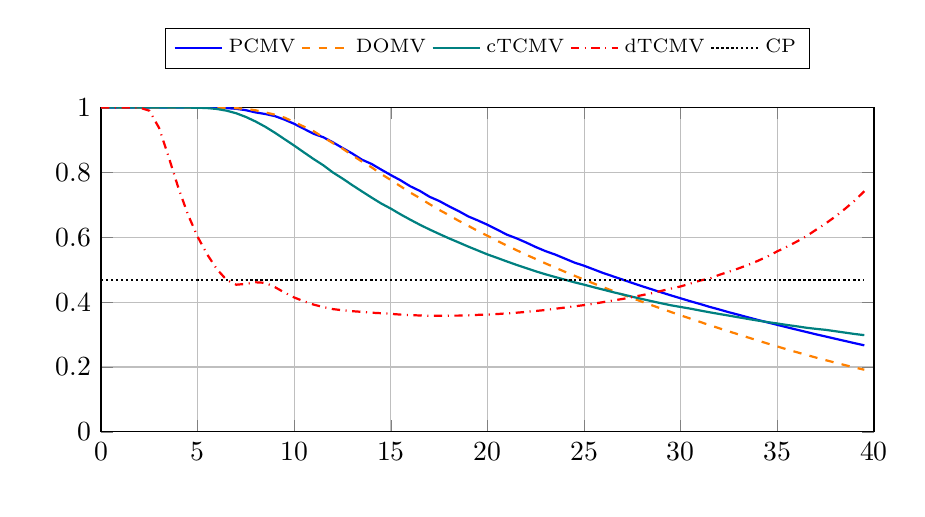
\begin{tikzpicture}\begin{axis}[width=.94\textwidth,height=57mm,xmin=0,xmax=40,ymin=0,ymax=1,xlabel={経過年},ylabel={平均リスク資産比率},legend columns=5,legend style={at={(.5,1.12)},anchor=south,font=\scriptsize},grid=major]
\addplot[blue,solid,thick] coordinates {(0.0000,1.000000) (0.5000,1.000000) (1.0000,1.000000) (1.5000,1.000000) (2.0000,1.000000) (2.5000,1.000000) (3.0000,1.000000) (3.5000,1.000000) (4.0000,1.000000) (4.5000,0.999997) (5.0000,0.999958) (5.5000,0.999834) (6.0000,0.999511) (6.5000,0.998516) (7.0000,0.996198) (7.5000,0.991926) (8.0000,0.985158) (8.5000,0.980227) (9.0000,0.973687) (9.5000,0.962742) (10.0000,0.949844) (10.5000,0.934534) (11.0000,0.919190) (11.5000,0.908667) (12.0000,0.892912) (12.5000,0.875404) (13.0000,0.858495) (13.5000,0.839469) (14.0000,0.826262) (14.5000,0.808757) (15.0000,0.791726) (15.5000,0.775821) (16.0000,0.757497) (16.5000,0.743096) (17.0000,0.725027) (17.5000,0.712033) (18.0000,0.695889) (18.5000,0.681045) (19.0000,0.664571) (19.5000,0.652031) (20.0000,0.638677) (20.5000,0.623677) (21.0000,0.608287) (21.5000,0.596925) (22.0000,0.583966) (22.5000,0.569960) (23.0000,0.557425) (23.5000,0.546863) (24.0000,0.534472) (24.5000,0.522085) (25.0000,0.512230) (25.5000,0.500986) (26.0000,0.489549) (26.5000,0.479556) (27.0000,0.469407) (27.5000,0.459029) (28.0000,0.449086) (28.5000,0.439666) (29.0000,0.429990) (29.5000,0.420791) (30.0000,0.411810) (30.5000,0.402790) (31.0000,0.394372) (31.5000,0.385420) (32.0000,0.377343) (32.5000,0.368832) (33.0000,0.361040) (33.5000,0.352950) (34.0000,0.345099) (34.5000,0.337527) (35.0000,0.329944) (35.5000,0.322550) (36.0000,0.315266) (36.5000,0.308079) (37.0000,0.300852) (37.5000,0.294107) (38.0000,0.287190) (38.5000,0.280397) (39.0000,0.273522) (39.5000,0.266902)};\addlegendentry{PCMV}
\addplot[orange,dashed,thick] coordinates {(0.0000,1.000000) (0.5000,1.000000) (1.0000,1.000000) (1.5000,1.000000) (2.0000,1.000000) (2.5000,1.000000) (3.0000,1.000000) (3.5000,1.000000) (4.0000,1.000000) (4.5000,1.000000) (5.0000,0.999997) (5.5000,0.999973) (6.0000,0.999834) (6.5000,0.999336) (7.0000,0.998120) (7.5000,0.996106) (8.0000,0.991665) (8.5000,0.985282) (9.0000,0.978074) (9.5000,0.968982) (10.0000,0.955226) (10.5000,0.941231) (11.0000,0.927211) (11.5000,0.908584) (12.0000,0.890427) (12.5000,0.873503) (13.0000,0.852958) (13.5000,0.833744) (14.0000,0.815880) (14.5000,0.795165) (15.0000,0.776586) (15.5000,0.757349) (16.0000,0.738168) (16.5000,0.720851) (17.0000,0.702316) (17.5000,0.684613) (18.0000,0.668407) (18.5000,0.651253) (19.0000,0.635724) (19.5000,0.619468) (20.0000,0.604625) (20.5000,0.589297) (21.0000,0.574589) (21.5000,0.560371) (22.0000,0.546294) (22.5000,0.533005) (23.0000,0.519612) (23.5000,0.506660) (24.0000,0.493864) (24.5000,0.481580) (25.0000,0.469378) (25.5000,0.457582) (26.0000,0.445798) (26.5000,0.434337) (27.0000,0.423070) (27.5000,0.412227) (28.0000,0.401290) (28.5000,0.390516) (29.0000,0.379899) (29.5000,0.369585) (30.0000,0.359430) (30.5000,0.349200) (31.0000,0.339094) (31.5000,0.328998) (32.0000,0.319316) (32.5000,0.309767) (33.0000,0.300383) (33.5000,0.290903) (34.0000,0.281641) (34.5000,0.272314) (35.0000,0.263397) (35.5000,0.254293) (36.0000,0.245825) (36.5000,0.237438) (37.0000,0.229112) (37.5000,0.221181) (38.0000,0.213499) (38.5000,0.205880) (39.0000,0.198517) (39.5000,0.191670)};\addlegendentry{DOMV}
\addplot[teal,solid,thick] coordinates {(0.0000,1.000000) (0.5000,1.000000) (1.0000,1.000000) (1.5000,1.000000) (2.0000,1.000000) (2.5000,1.000000) (3.0000,1.000000) (3.5000,1.000000) (4.0000,0.999997) (4.5000,0.999959) (5.0000,0.999652) (5.5000,0.998501) (6.0000,0.995673) (6.5000,0.990467) (7.0000,0.982398) (7.5000,0.971044) (8.0000,0.957031) (8.5000,0.940887) (9.0000,0.922385) (9.5000,0.902414) (10.0000,0.882757) (10.5000,0.861863) (11.0000,0.841400) (11.5000,0.822263) (12.0000,0.799966) (12.5000,0.781096) (13.0000,0.760980) (13.5000,0.741613) (14.0000,0.722574) (14.5000,0.704262) (15.0000,0.688349) (15.5000,0.670796) (16.0000,0.654438) (16.5000,0.638748) (17.0000,0.624147) (17.5000,0.610418) (18.0000,0.596972) (18.5000,0.584388) (19.0000,0.571511) (19.5000,0.559378) (20.0000,0.547183) (20.5000,0.536594) (21.0000,0.525613) (21.5000,0.515036) (22.0000,0.505105) (22.5000,0.495037) (23.0000,0.486016) (23.5000,0.477587) (24.0000,0.469345) (24.5000,0.461229) (25.0000,0.453928) (25.5000,0.446008) (26.0000,0.438504) (26.5000,0.430759) (27.0000,0.423781) (27.5000,0.416666) (28.0000,0.409688) (28.5000,0.403011) (29.0000,0.396473) (29.5000,0.390302) (30.0000,0.385149) (30.5000,0.380001) (31.0000,0.374284) (31.5000,0.368706) (32.0000,0.363543) (32.5000,0.358476) (33.0000,0.353215) (33.5000,0.348132) (34.0000,0.343148) (34.5000,0.338484) (35.0000,0.334260) (35.5000,0.329634) (36.0000,0.325632) (36.5000,0.321170) (37.0000,0.317696) (37.5000,0.314692) (38.0000,0.310417) (38.5000,0.306157) (39.0000,0.301846) (39.5000,0.298371)};\addlegendentry{cTCMV}
\addplot[red,dashdotted,thick] coordinates {(0.0000,1.000000) (0.5000,1.000000) (1.0000,1.000000) (1.5000,1.000000) (2.0000,0.999866) (2.5000,0.990412) (3.0000,0.937818) (3.5000,0.847588) (4.0000,0.752777) (4.5000,0.669715) (5.0000,0.601514) (5.5000,0.546462) (6.0000,0.501410) (6.5000,0.468415) (7.0000,0.453853) (7.5000,0.456436) (8.0000,0.461218) (8.5000,0.459701) (9.0000,0.446234) (9.5000,0.429531) (10.0000,0.414349) (10.5000,0.402724) (11.0000,0.392515) (11.5000,0.384868) (12.0000,0.378603) (12.5000,0.375089) (13.0000,0.372180) (13.5000,0.370111) (14.0000,0.367499) (14.5000,0.365936) (15.0000,0.363932) (15.5000,0.361667) (16.0000,0.360010) (16.5000,0.359005) (17.0000,0.357977) (17.5000,0.358261) (18.0000,0.358455) (18.5000,0.358564) (19.0000,0.359150) (19.5000,0.360854) (20.0000,0.361941) (20.5000,0.363395) (21.0000,0.365491) (21.5000,0.367521) (22.0000,0.369989) (22.5000,0.372831) (23.0000,0.375930) (23.5000,0.379700) (24.0000,0.383316) (24.5000,0.387147) (25.0000,0.390989) (25.5000,0.395312) (26.0000,0.400327) (26.5000,0.405336) (27.0000,0.410024) (27.5000,0.415764) (28.0000,0.421596) (28.5000,0.427745) (29.0000,0.434835) (29.5000,0.441837) (30.0000,0.448623) (30.5000,0.457502) (31.0000,0.466617) (31.5000,0.472857) (32.0000,0.484387) (32.5000,0.493923) (33.0000,0.504261) (33.5000,0.515308) (34.0000,0.527700) (34.5000,0.541424) (35.0000,0.556872) (35.5000,0.571257) (36.0000,0.586654) (36.5000,0.603250) (37.0000,0.623135) (37.5000,0.642594) (38.0000,0.664091) (38.5000,0.687770) (39.0000,0.713058) (39.5000,0.742180)};\addlegendentry{dTCMV}
\addplot[black,densely dotted,thick] coordinates {(0.0000,0.468884) (0.5000,0.468884) (1.0000,0.468884) (1.5000,0.468884) (2.0000,0.468884) (2.5000,0.468884) (3.0000,0.468884) (3.5000,0.468884) (4.0000,0.468884) (4.5000,0.468884) (5.0000,0.468884) (5.5000,0.468884) (6.0000,0.468884) (6.5000,0.468884) (7.0000,0.468884) (7.5000,0.468884) (8.0000,0.468884) (8.5000,0.468884) (9.0000,0.468884) (9.5000,0.468884) (10.0000,0.468884) (10.5000,0.468884) (11.0000,0.468884) (11.5000,0.468884) (12.0000,0.468884) (12.5000,0.468884) (13.0000,0.468884) (13.5000,0.468884) (14.0000,0.468884) (14.5000,0.468884) (15.0000,0.468884) (15.5000,0.468884) (16.0000,0.468884) (16.5000,0.468884) (17.0000,0.468884) (17.5000,0.468884) (18.0000,0.468884) (18.5000,0.468884) (19.0000,0.468884) (19.5000,0.468884) (20.0000,0.468884) (20.5000,0.468884) (21.0000,0.468884) (21.5000,0.468884) (22.0000,0.468884) (22.5000,0.468884) (23.0000,0.468884) (23.5000,0.468884) (24.0000,0.468884) (24.5000,0.468884) (25.0000,0.468884) (25.5000,0.468884) (26.0000,0.468884) (26.5000,0.468884) (27.0000,0.468884) (27.5000,0.468884) (28.0000,0.468884) (28.5000,0.468884) (29.0000,0.468884) (29.5000,0.468884) (30.0000,0.468884) (30.5000,0.468884) (31.0000,0.468884) (31.5000,0.468884) (32.0000,0.468884) (32.5000,0.468884) (33.0000,0.468884) (33.5000,0.468884) (34.0000,0.468884) (34.5000,0.468884) (35.0000,0.468884) (35.5000,0.468884) (36.0000,0.468884) (36.5000,0.468884) (37.0000,0.468884) (37.5000,0.468884) (38.0000,0.468884) (38.5000,0.468884) (39.0000,0.468884) (39.5000,0.468884)};\addlegendentry{CP}
\end{axis}\end{tikzpicture}\caption{共通期待終価へ再較正した方策の平均配分（独立評価）}\label{fig:recalibrated_glide}\end{figure}
\begin{figure}[htbp]\centering
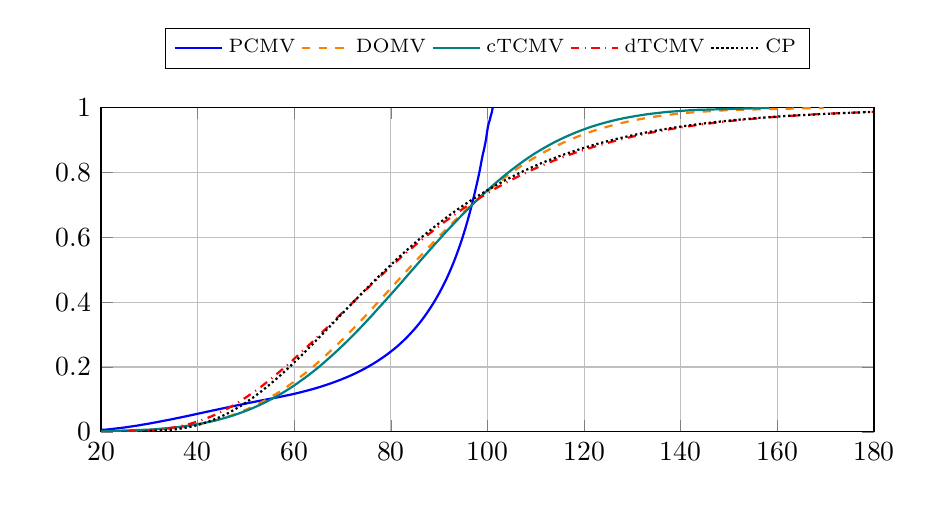
\begin{tikzpicture}\begin{axis}[width=.94\textwidth,height=57mm,xmin=20,xmax=180,ymin=0,ymax=1,xlabel={退職時残高},ylabel={累積確率},legend columns=5,legend style={at={(.5,1.12)},anchor=south,font=\scriptsize},grid=major]
\addplot[blue,solid,thick] coordinates {(14.54044,0.00100) (21.26815,0.00724) (24.80582,0.01348) (27.61882,0.01971) (30.07038,0.02595) (32.31261,0.03219) (34.45746,0.03843) (36.48407,0.04466) (38.48385,0.05090) (40.38487,0.05714) (42.32072,0.06338) (44.29707,0.06961) (46.25348,0.07585) (48.26917,0.08209) (50.29260,0.08833) (52.38174,0.09456) (54.54832,0.10080) (56.70403,0.10704) (58.76413,0.11328) (60.60467,0.11951) (62.26973,0.12575) (63.83098,0.13199) (65.23647,0.13822) (66.54945,0.14446) (67.75956,0.15070) (68.91629,0.15694) (69.97458,0.16318) (70.99622,0.16941) (71.95314,0.17565) (72.84192,0.18189) (73.68715,0.18812) (74.47510,0.19436) (75.24109,0.20060) (75.96690,0.20684) (76.66381,0.21308) (77.31589,0.21931) (77.95280,0.22555) (78.55665,0.23179) (79.14030,0.23802) (79.69594,0.24426) (80.23594,0.25050) (80.76344,0.25674) (81.25631,0.26298) (81.72858,0.26921) (82.18045,0.27545) (82.63279,0.28169) (83.06583,0.28792) (83.47903,0.29416) (83.86716,0.30040) (84.26086,0.30664) (84.64403,0.31288) (85.00963,0.31911) (85.36846,0.32535) (85.71442,0.33159) (86.04725,0.33782) (86.36684,0.34406) (86.68368,0.35030) (86.99141,0.35654) (87.28366,0.36278) (87.56872,0.36901) (87.85241,0.37525) (88.12852,0.38149) (88.40048,0.38772) (88.66590,0.39396) (88.92741,0.40020) (89.18218,0.40644) (89.42532,0.41268) (89.65950,0.41891) (89.89268,0.42515) (90.12283,0.43139) (90.34747,0.43762) (90.57027,0.44386) (90.78640,0.45010) (90.99704,0.45634) (91.20566,0.46258) (91.41045,0.46881) (91.60533,0.47505) (91.79946,0.48129) (91.98688,0.48752) (92.17328,0.49376) (92.35008,0.50000) (92.52819,0.50624) (92.70457,0.51248) (92.87413,0.51871) (93.03896,0.52495) (93.20608,0.53119) (93.36610,0.53743) (93.52287,0.54366) (93.67801,0.54990) (93.83002,0.55614) (93.98069,0.56237) (94.12927,0.56861) (94.27537,0.57485) (94.41762,0.58109) (94.55903,0.58732) (94.69764,0.59356) (94.83492,0.59980) (94.96712,0.60604) (95.09932,0.61228) (95.22853,0.61851) (95.35742,0.62475) (95.48075,0.63099) (95.60309,0.63723) (95.72376,0.64346) (95.84260,0.64970) (95.95842,0.65594) (96.07541,0.66217) (96.18940,0.66841) (96.30398,0.67465) (96.41523,0.68089) (96.52727,0.68712) (96.63400,0.69336) (96.74000,0.69960) (96.84417,0.70584) (96.94900,0.71208) (97.05270,0.71831) (97.15578,0.72455) (97.25782,0.73079) (97.35641,0.73703) (97.45411,0.74326) (97.55017,0.74950) (97.64662,0.75574) (97.74387,0.76197) (97.83915,0.76821) (97.93704,0.77445) (98.02964,0.78069) (98.11765,0.78692) (98.20666,0.79316) (98.29520,0.79940) (98.38250,0.80564) (98.46664,0.81188) (98.54629,0.81811) (98.62279,0.82435) (98.69823,0.83059) (98.77659,0.83683) (98.85529,0.84306) (98.94055,0.84930) (99.03165,0.85554) (99.12779,0.86177) (99.22570,0.86801) (99.31699,0.87425) (99.40105,0.88049) (99.48378,0.88672) (99.57113,0.89296) (99.65420,0.89920) (99.72364,0.90544) (99.78517,0.91168) (99.84288,0.91791) (99.90342,0.92415) (99.96915,0.93039) (100.03973,0.93663) (100.11982,0.94286) (100.21068,0.94910) (100.32246,0.95534) (100.46907,0.96157) (100.56887,0.96781) (100.66183,0.97405) (100.78812,0.98029) (100.92998,0.98652) (100.97778,0.99276) (101.07678,0.99900)};\addlegendentry{PCMV}
\addplot[orange,dashed,thick] coordinates {(22.43520,0.00100) (32.27026,0.00724) (36.24813,0.01348) (38.97120,0.01971) (41.09646,0.02595) (42.92490,0.03219) (44.44385,0.03843) (45.79243,0.04466) (47.03881,0.05090) (48.15640,0.05714) (49.17124,0.06338) (50.18032,0.06961) (51.09909,0.07585) (52.00111,0.08209) (52.82207,0.08833) (53.60177,0.09456) (54.37090,0.10080) (55.09413,0.10704) (55.80943,0.11328) (56.49956,0.11951) (57.14490,0.12575) (57.77056,0.13199) (58.40800,0.13822) (58.98481,0.14446) (59.57225,0.15070) (60.17346,0.15694) (60.72773,0.16318) (61.25616,0.16941) (61.79076,0.17565) (62.33159,0.18189) (62.84008,0.18812) (63.33563,0.19436) (63.84276,0.20060) (64.33925,0.20684) (64.81413,0.21308) (65.28511,0.21931) (65.74529,0.22555) (66.22145,0.23179) (66.67815,0.23802) (67.10898,0.24426) (67.56181,0.25050) (68.01944,0.25674) (68.47326,0.26298) (68.90815,0.26921) (69.32992,0.27545) (69.75298,0.28169) (70.19007,0.28792) (70.61370,0.29416) (71.02305,0.30040) (71.42313,0.30664) (71.84001,0.31288) (72.26244,0.31911) (72.66979,0.32535) (73.06411,0.33159) (73.46111,0.33782) (73.86529,0.34406) (74.27351,0.35030) (74.66613,0.35654) (75.05200,0.36278) (75.42599,0.36901) (75.81643,0.37525) (76.20580,0.38149) (76.59236,0.38772) (76.96482,0.39396) (77.34004,0.40020) (77.72946,0.40644) (78.12024,0.41268) (78.50716,0.41891) (78.88936,0.42515) (79.27082,0.43139) (79.65983,0.43762) (80.05205,0.44386) (80.43678,0.45010) (80.81137,0.45634) (81.19010,0.46258) (81.56889,0.46881) (81.96741,0.47505) (82.35566,0.48129) (82.73094,0.48752) (83.10128,0.49376) (83.47603,0.50000) (83.86322,0.50624) (84.25153,0.51248) (84.63819,0.51871) (85.02082,0.52495) (85.40605,0.53119) (85.79938,0.53743) (86.19925,0.54366) (86.59248,0.54990) (86.98299,0.55614) (87.37271,0.56237) (87.77839,0.56861) (88.18204,0.57485) (88.58201,0.58109) (88.97855,0.58732) (89.38285,0.59356) (89.78048,0.59980) (90.18649,0.60604) (90.59783,0.61228) (91.00537,0.61851) (91.41387,0.62475) (91.83783,0.63099) (92.25915,0.63723) (92.69259,0.64346) (93.10540,0.64970) (93.53162,0.65594) (93.97049,0.66217) (94.42145,0.66841) (94.87136,0.67465) (95.31815,0.68089) (95.77964,0.68712) (96.24577,0.69336) (96.71168,0.69960) (97.17581,0.70584) (97.65124,0.71208) (98.14158,0.71831) (98.61743,0.72455) (99.10630,0.73079) (99.60243,0.73703) (100.11785,0.74326) (100.61791,0.74950) (101.12156,0.75574) (101.63562,0.76197) (102.17357,0.76821) (102.70757,0.77445) (103.25292,0.78069) (103.81709,0.78692) (104.40431,0.79316) (104.97364,0.79940) (105.55739,0.80564) (106.16784,0.81188) (106.77584,0.81811) (107.40369,0.82435) (108.07499,0.83059) (108.75609,0.83683) (109.43858,0.84306) (110.15713,0.84930) (110.87855,0.85554) (111.62711,0.86177) (112.41991,0.86801) (113.22669,0.87425) (114.07299,0.88049) (114.93616,0.88672) (115.86178,0.89296) (116.79678,0.89920) (117.79076,0.90544) (118.84294,0.91168) (119.96697,0.91791) (121.13700,0.92415) (122.38806,0.93039) (123.74890,0.93663) (125.19709,0.94286) (126.82433,0.94910) (128.58658,0.95534) (130.56027,0.96157) (132.86686,0.96781) (135.51260,0.97405) (138.86027,0.98029) (143.37523,0.98652) (150.33677,0.99276) (169.58230,0.99900)};\addlegendentry{DOMV}
\addplot[teal,solid,thick] coordinates {(18.98950,0.00100) (30.52149,0.00724) (35.17547,0.01348) (38.35159,0.01971) (40.80425,0.02595) (42.81350,0.03219) (44.50900,0.03843) (46.02585,0.04466) (47.35324,0.05090) (48.59456,0.05714) (49.72732,0.06338) (50.79792,0.06961) (51.77709,0.07585) (52.70712,0.08209) (53.59815,0.08833) (54.44039,0.09456) (55.23412,0.10080) (56.01002,0.10704) (56.75852,0.11328) (57.48155,0.11951) (58.17370,0.12575) (58.83899,0.13199) (59.48592,0.13822) (60.11876,0.14446) (60.71133,0.15070) (61.29106,0.15694) (61.87913,0.16318) (62.44934,0.16941) (63.00614,0.17565) (63.54985,0.18189) (64.08993,0.18812) (64.61012,0.19436) (65.11613,0.20060) (65.60720,0.20684) (66.08469,0.21308) (66.57188,0.21931) (67.05563,0.22555) (67.52500,0.23179) (67.98551,0.23802) (68.44216,0.24426) (68.89520,0.25050) (69.33826,0.25674) (69.78165,0.26298) (70.22570,0.26921) (70.65628,0.27545) (71.08094,0.28169) (71.49876,0.28792) (71.91771,0.29416) (72.33492,0.30040) (72.75166,0.30664) (73.16207,0.31288) (73.56045,0.31911) (73.96108,0.32535) (74.35651,0.33159) (74.74958,0.33782) (75.14533,0.34406) (75.52859,0.35030) (75.91528,0.35654) (76.30210,0.36278) (76.67706,0.36901) (77.04946,0.37525) (77.42351,0.38149) (77.80349,0.38772) (78.18325,0.39396) (78.56364,0.40020) (78.94093,0.40644) (79.31064,0.41268) (79.68630,0.41891) (80.06429,0.42515) (80.43945,0.43139) (80.81247,0.43762) (81.18318,0.44386) (81.54909,0.45010) (81.91994,0.45634) (82.28878,0.46258) (82.64885,0.46881) (83.00649,0.47505) (83.36620,0.48129) (83.73457,0.48752) (84.09347,0.49376) (84.46737,0.50000) (84.83576,0.50624) (85.18987,0.51248) (85.55238,0.51871) (85.92541,0.52495) (86.29261,0.53119) (86.66319,0.53743) (87.03021,0.54366) (87.40009,0.54990) (87.76542,0.55614) (88.13483,0.56237) (88.50410,0.56861) (88.88189,0.57485) (89.25561,0.58109) (89.63252,0.58732) (90.00487,0.59356) (90.37978,0.59980) (90.76074,0.60604) (91.14376,0.61228) (91.52242,0.61851) (91.90326,0.62475) (92.29869,0.63099) (92.69531,0.63723) (93.09291,0.64346) (93.49683,0.64970) (93.89728,0.65594) (94.29367,0.66217) (94.69828,0.66841) (95.11318,0.67465) (95.52452,0.68089) (95.93736,0.68712) (96.36361,0.69336) (96.77982,0.69960) (97.20022,0.70584) (97.63074,0.71208) (98.06751,0.71831) (98.50523,0.72455) (98.94878,0.73079) (99.40013,0.73703) (99.85990,0.74326) (100.32684,0.74950) (100.79731,0.75574) (101.27013,0.76197) (101.75044,0.76821) (102.23941,0.77445) (102.73294,0.78069) (103.23454,0.78692) (103.75418,0.79316) (104.26851,0.79940) (104.79941,0.80564) (105.34684,0.81188) (105.89445,0.81811) (106.45344,0.82435) (107.03318,0.83059) (107.62064,0.83683) (108.22061,0.84306) (108.84222,0.84930) (109.47519,0.85554) (110.13359,0.86177) (110.83112,0.86801) (111.55090,0.87425) (112.28766,0.88049) (113.04346,0.88672) (113.82468,0.89296) (114.65995,0.89920) (115.52639,0.90544) (116.44217,0.91168) (117.40506,0.91791) (118.41170,0.92415) (119.49807,0.93039) (120.65737,0.93663) (121.90069,0.94286) (123.25939,0.94910) (124.77727,0.95534) (126.44700,0.96157) (128.35694,0.96781) (130.67235,0.97405) (133.41472,0.98029) (137.06405,0.98652) (142.77142,0.99276) (158.22203,0.99900)};\addlegendentry{cTCMV}
\addplot[red,dashdotted,thick] coordinates {(25.43111,0.00100) (32.15502,0.00724) (34.98973,0.01348) (37.03777,0.01971) (38.64775,0.02595) (40.02304,0.03219) (41.24743,0.03843) (42.31641,0.04466) (43.31488,0.05090) (44.22578,0.05714) (45.08050,0.06338) (45.89763,0.06961) (46.65805,0.07585) (47.40763,0.08209) (48.09999,0.08833) (48.77535,0.09456) (49.42105,0.10080) (50.05888,0.10704) (50.68153,0.11328) (51.29733,0.11951) (51.87935,0.12575) (52.46435,0.13199) (53.03271,0.13822) (53.56858,0.14446) (54.10206,0.15070) (54.62543,0.15694) (55.14316,0.16318) (55.64612,0.16941) (56.15730,0.17565) (56.65506,0.18189) (57.15016,0.18812) (57.64012,0.19436) (58.12357,0.20060) (58.60087,0.20684) (59.07472,0.21308) (59.53977,0.21931) (59.99850,0.22555) (60.45993,0.23179) (60.90926,0.23802) (61.36459,0.24426) (61.80579,0.25050) (62.24936,0.25674) (62.70543,0.26298) (63.14612,0.26921) (63.59169,0.27545) (64.02272,0.28169) (64.44873,0.28792) (64.87622,0.29416) (65.31091,0.30040) (65.74068,0.30664) (66.17252,0.31288) (66.60695,0.31911) (67.04228,0.32535) (67.47104,0.33159) (67.89258,0.33782) (68.32432,0.34406) (68.75602,0.35030) (69.17494,0.35654) (69.60121,0.36278) (70.03274,0.36901) (70.46113,0.37525) (70.89212,0.38149) (71.31997,0.38772) (71.75129,0.39396) (72.18354,0.40020) (72.60814,0.40644) (73.04339,0.41268) (73.47897,0.41891) (73.92207,0.42515) (74.35394,0.43139) (74.79074,0.43762) (75.22860,0.44386) (75.66522,0.45010) (76.10536,0.45634) (76.54501,0.46258) (76.99032,0.46881) (77.43795,0.47505) (77.89436,0.48129) (78.35232,0.48752) (78.80422,0.49376) (79.25811,0.50000) (79.71924,0.50624) (80.16819,0.51248) (80.63291,0.51871) (81.09533,0.52495) (81.56658,0.53119) (82.03429,0.53743) (82.51136,0.54366) (83.00194,0.54990) (83.49644,0.55614) (83.98563,0.56237) (84.47606,0.56861) (84.97127,0.57485) (85.46975,0.58109) (85.96880,0.58732) (86.47881,0.59356) (86.99980,0.59980) (87.53339,0.60604) (88.05249,0.61228) (88.58521,0.61851) (89.11786,0.62475) (89.66739,0.63099) (90.21373,0.63723) (90.76680,0.64346) (91.31213,0.64970) (91.87896,0.65594) (92.44547,0.66217) (93.03012,0.66841) (93.62700,0.67465) (94.22970,0.68089) (94.83061,0.68712) (95.44615,0.69336) (96.08066,0.69960) (96.73471,0.70584) (97.39081,0.71208) (98.05605,0.71831) (98.72480,0.72455) (99.41369,0.73079) (100.10591,0.73703) (100.80690,0.74326) (101.52059,0.74950) (102.25989,0.75574) (103.02647,0.76197) (103.79146,0.76821) (104.58318,0.77445) (105.40870,0.78069) (106.27283,0.78692) (107.11635,0.79316) (107.98636,0.79940) (108.87426,0.80564) (109.81686,0.81188) (110.75502,0.81811) (111.73788,0.82435) (112.74528,0.83059) (113.78502,0.83683) (114.85254,0.84306) (115.98600,0.84930) (117.15040,0.85554) (118.35286,0.86177) (119.61078,0.86801) (120.93458,0.87425) (122.31902,0.88049) (123.80970,0.88672) (125.31639,0.89296) (126.90235,0.89920) (128.60142,0.90544) (130.38259,0.91168) (132.30770,0.91791) (134.36368,0.92415) (136.64475,0.93039) (139.10165,0.93663) (141.78351,0.94286) (144.81257,0.94910) (148.21326,0.95534) (152.09698,0.96157) (156.63274,0.96781) (162.13084,0.97405) (169.16693,0.98029) (178.80874,0.98652) (194.42785,0.99276) (245.43443,0.99900)};\addlegendentry{dTCMV}
\addplot[black,densely dotted,thick] coordinates {(29.06529,0.00100) (35.19185,0.00724) (37.76877,0.01348) (39.63526,0.01971) (41.09739,0.02595) (42.34781,0.03219) (43.44116,0.03843) (44.43043,0.04466) (45.35140,0.05090) (46.20726,0.05714) (46.99478,0.06338) (47.72539,0.06961) (48.43710,0.07585) (49.10743,0.08209) (49.76134,0.08833) (50.38012,0.09456) (50.98678,0.10080) (51.57183,0.10704) (52.13878,0.11328) (52.69064,0.11951) (53.23347,0.12575) (53.75459,0.13199) (54.26868,0.13822) (54.78503,0.14446) (55.29262,0.15070) (55.77754,0.15694) (56.26309,0.16318) (56.74107,0.16941) (57.20696,0.17565) (57.67313,0.18189) (58.12815,0.18812) (58.58313,0.19436) (59.03115,0.20060) (59.47047,0.20684) (59.91228,0.21308) (60.34082,0.21931) (60.77686,0.22555) (61.21549,0.23179) (61.62859,0.23802) (62.04282,0.24426) (62.46276,0.25050) (62.87581,0.25674) (63.29015,0.26298) (63.70206,0.26921) (64.10961,0.27545) (64.51455,0.28169) (64.93518,0.28792) (65.33604,0.29416) (65.74581,0.30040) (66.15232,0.30664) (66.55996,0.31288) (66.96327,0.31911) (67.37327,0.32535) (67.77089,0.33159) (68.17488,0.33782) (68.57972,0.34406) (68.98161,0.35030) (69.38446,0.35654) (69.77861,0.36278) (70.18855,0.36901) (70.60038,0.37525) (71.00570,0.38149) (71.41383,0.38772) (71.81642,0.39396) (72.22820,0.40020) (72.63986,0.40644) (73.03757,0.41268) (73.43239,0.41891) (73.84772,0.42515) (74.26011,0.43139) (74.68322,0.43762) (75.10217,0.44386) (75.52133,0.45010) (75.94002,0.45634) (76.36239,0.46258) (76.79052,0.46881) (77.21401,0.47505) (77.64361,0.48129) (78.07355,0.48752) (78.50354,0.49376) (78.92994,0.50000) (79.36400,0.50624) (79.79919,0.51248) (80.24457,0.51871) (80.69395,0.52495) (81.13736,0.53119) (81.58946,0.53743) (82.04474,0.54366) (82.50279,0.54990) (82.96291,0.55614) (83.43442,0.56237) (83.90868,0.56861) (84.38164,0.57485) (84.86130,0.58109) (85.33834,0.58732) (85.82922,0.59356) (86.32686,0.59980) (86.82066,0.60604) (87.34057,0.61228) (87.85571,0.61851) (88.37793,0.62475) (88.90485,0.63099) (89.43044,0.63723) (89.97667,0.64346) (90.51927,0.64970) (91.06107,0.65594) (91.60516,0.66217) (92.16335,0.66841) (92.72765,0.67465) (93.31149,0.68089) (93.90451,0.68712) (94.51846,0.69336) (95.13016,0.69960) (95.75357,0.70584) (96.38727,0.71208) (97.03131,0.71831) (97.69638,0.72455) (98.35993,0.73079) (99.05373,0.73703) (99.75502,0.74326) (100.47765,0.74950) (101.20451,0.75574) (101.93469,0.76197) (102.70122,0.76821) (103.46538,0.77445) (104.27270,0.78069) (105.08817,0.78692) (105.92037,0.79316) (106.78044,0.79940) (107.66394,0.80564) (108.57476,0.81188) (109.51594,0.81811) (110.46821,0.82435) (111.46385,0.83059) (112.53587,0.83683) (113.58643,0.84306) (114.71713,0.84930) (115.85283,0.85554) (117.08001,0.86177) (118.32741,0.86801) (119.62546,0.87425) (120.98708,0.88049) (122.40440,0.88672) (123.93570,0.89296) (125.55257,0.89920) (127.27930,0.90544) (129.10418,0.91168) (131.02858,0.91791) (133.12611,0.92415) (135.41631,0.93039) (137.93765,0.93663) (140.65508,0.94286) (143.71339,0.94910) (147.14648,0.95534) (151.16671,0.96157) (155.83420,0.96781) (161.65393,0.97405) (169.18109,0.98029) (179.20985,0.98652) (196.34787,0.99276) (252.48025,0.99900)};\addlegendentry{CP}
\end{axis}\end{tikzpicture}\caption{共通期待終価へ再較正した方策の終価分布（独立評価）}\label{fig:recalibrated_cdf}\end{figure}


\section{状態別退職成果と年金実務への翻訳}
\noindent 以下の状態別数値は第\ref{sec:equalmean}節の再較正方策ではなく，前節までの保存方策監査に対応する歴史的比較である．\par
\label{sec:rolling}
\subsection{同じ残高から将来方策を比較する}
Markov方策$j$について，$\mu_j(t,x)=\E_{t,x}[W_T^j]$，$v_j(t,x)=\Var_{t,x}(W_T^j)$とすると
\begin{equation}
\Var(W_T^j)=\E[v_j(t,X_t^j)]+\Var(\mu_j(t,X_t^j)).
\label{eq:totalvar}
\end{equation}
これは全分散の公式であり，新しいリスク分解定理ではない．時点0では未実現の残高シナリオを評価し，途中評価では実現残高を所与として将来の分布を評価する．両者は異なる問いに答える．共通市場ショックを受ける実際の加入者集団の横断的格差と，単一加入者のシナリオ間のばらつきも区別する．

\begin{table}[htbp]\centering\footnotesize
\caption{同じ途中状態からの条件付き退職成果（各10万経路）}\label{tab:rolling}
\begin{tabular}{llrrrrr}
\toprule
開始状態 & 方策 & 平均 & 標準偏差 & q05 & LCVaR & q95 \\ \midrule
30年・残高45.268 & cTCMV保存 & 72.44 & 13.11 & 51.21 & 46.37 & 94.60 \\
 & dTCMV保存 & 81.46 & 31.43 & 41.05 & 35.50 & 140.62 \\
30年・残高67.412 & cTCMV保存 & 98.84 & 14.00 & 76.28 & 70.81 & 121.88 \\
 & dTCMV保存 & 114.53 & 44.54 & 57.82 & 49.92 & 196.47 \\
35年・残高36.200 & cTCMV保存 & 48.29 & 8.32 & 35.16 & 31.94 & 62.39 \\
 & dTCMV保存 & 51.35 & 16.31 & 29.46 & 26.51 & 81.38 \\
\bottomrule\end{tabular}
\par\vspace{3pt}\begin{minipage}{0.97\textwidth}\footnotesize LCVaRは下位5\%平均富．時点と残高を固定して保存方策を継続した結果．条件付き平均の再較正は行っていない．\end{minipage}
\end{table}
表\ref{tab:rolling}は，参照版の代表状態を固定し，cTCMV・dTCMVの保存方策を10万経路で再評価した結果である．状態選択は網羅的ではなく，二方策の条件付き平均もそろえていない．30年・中位残高では，dTCMV保存方策は平均を約9.03高める一方，LCVaRを約10.87下げる．35年・低残高でも，平均上昇と下位裾悪化が同時に現れる．これは無償の成果改善ではなく，追加リスクと期待成果の交換である．

\subsection{残高を退職所得と不足額へ変換する}
終端富の単位は「年間拠出額を1」とする．実務では，年間拠出額を$C$円，退職時点の年金現価係数を確定値$\mathfrak a_T>0$とした説明用換算
\begin{equation}
I_T=\frac{CW_T}{\mathfrak a_T}
\label{eq:income}
\end{equation}
により年額所得へ直せる．$\mathfrak a_T$が一定なら，平均，分位点，LCVaRはすべて$C/\mathfrak a_T$倍となる．確率的な年金化価格ではこの単純換算はできない．$D_T$に既存DBの年金現価を含めた場合，所得換算後に同じDB給付を二重加算しない．

例として$C=30$万円，$\mathfrak a_T=20$という\emph{仮定上の換算}なら，富1は年額1.5万円に相当する．30年・中位残高でのdTCMVへの変更は，平均所得を約13.5万円/年高める一方，下位5\%平均所得を約16.3万円/年下げる交換となる．これは年金商品の見積りや市場の年金化率ではなく，表の差を理解するための例である．

富の目標$K$に対し，$p_K=\Pr(W_T<K)$と$e_K=\E[(K-W_T)_+]$も併記する．$K=60$を説明用の目標とした基準計算では，PCMV保存方策の不足確率は約12.58\%，cTCMVは約15.44\%だが，期待不足額はそれぞれ約2.46，1.65である．不足する頻度が少なくても，不足した際に深く落ち込むことがある．さらに35年・低残高では，cTCMVの不足確率約91.7\%に対しdTCMVは約74.5\%だが，下位裾はdTCMVの方が低い．不足確率だけで救済的な運用と位置づけることはできない．

\subsection{採用判断のための検証手順}
\label{sec:practice}
制度運営者は，特定の解概念を商品名へ直結させる前に，次の条件を運用仕様として定める．
\begin{enumerate}[leftmargin=2em,itemsep=3pt]
\item 退職所得目標，拠出の確実性，背景富の扱いおよび分散・不足額・下位裾の許容水準を決める．
\item 初期計画を維持するか，逐次見直すか，将来の自己との均衡を使うかを選ぶ．
\item PCMVのターゲットまたは選好係数をそろえ，直接制約方策とクリップを同じ評価モデルで比較する．
\item 解析特殊例，一段階残差，独立分布評価，残高・制御・時間格子，境界および共通平均較正を監査する．
\item 同じ加入者状態での期待所得と下方所得を説明し，手数料，売買可能商品，更新頻度を加えた結果で採用を判断する．
\end{enumerate}
例えば，年額所得のLCVaR差を許容幅$\varepsilon_I$以内とするなら，終端富の許容幅は$\varepsilon_W=\mathfrak a_T\varepsilon_I/C$となる．実務上の許容誤差を年金所得単位から決め，数値精度の採否へ戻す点に意味がある．閾値は加入者属性と制度目的に応じて定め，本稿の例示値を一律に採用しない．

cTCMVは定数係数のため説明しやすい候補，DOMVは残存期間問題を見直す候補，dTCMVは背景富を反映する候補である．しかし，これだけで標準デフォルト，定期見直し，個別化助言への最適な割当てが実証されたわけではない．PCMVにも拠出・残高を通じた状態依存性があり，個別化はdTCMVに固有ではない．複数方策を切り替える運用は別の方策となるため，切替後の分布を改めて評価する．

\section{限界と今後の研究}
\label{sec:limits}
第\ref{sec:equalmean}節で，共通有限モデル内の再最適化と期待終価84.78への再較正を実施した．残る課題は，連続時間・連続制御への誤差をさらに定量化することである．有限制御集合での全数探索，DOMVターゲット値の誤差上界，標本点における連続制御監査はそれぞれ保証範囲が異なる．月次モデルの数値比較を，すべての許容連続時間方策に対する厳密な順位の証明と解釈しない．

第二に，係数が既知という仮定を緩め，期待超過収益，変動性，インフレ，手数料の誤推定を含める必要がある．本稿のパラメータは例示値であり，特定市場の最新推定値ではない．第三に，確率的給与・拠出停止・死亡・複数資産を扱い，蓄積期と退職後取崩しを同じ所得目標で接続する．これらは所得状態や年金化価格などを追加する別の制御問題となる．

理論面では，制約付き均衡の大域存在・一意性，DOMVの共同可測なフィードバック選択と閉ループの適切性，離散均衡の連続時間収束が残る．正の歪度選好を持つMVSは，これらの基本的検証の後に位置づける（付録\ref{app:mvs}）．

\section{結論}
制約を満たすこと，制約付き最適化を再現すること，退職成果を正確に評価することは，三つの異なる要件である．本稿は四つの動的平均--分散解概念を整理し，固定ターゲット損失の残差表示，補間による追加分散，無制約係数のモーメント検証および独立分布評価を一つの検証手順へまとめた．

共通期待終価への再最適化では，分散と下位裾が異なる評価軸であることを再確認した．有限モデルの最適性と独立評価の数値精度を分け，較正係数・方策・検証データを公開する．参照計算では，内部モーメント一致があっても定率運用の分散精度に問題が残り，保存方策の共通平均較正も独立評価で維持されなかった．富依存係数の符号を確認したクリップ比較では，下位裾の差を一方向へ一般化できない．一方，同じ途中残高からの評価は，追加的な期待所得と下方リスクの交換を加入者に説明する具体的な材料となる．年金実務にとって重要なのは，複雑な方策を採用すること自体ではなく，採用する方策と説明する退職成果の双方について，独立に確認できる根拠を持つことである．

\appendix
\section{検証論証の条件と範囲}
\label{app:verify}
\subsection{非負状態と一様モーメント}
固定された進行可測な比率過程$u\in[0,1]$について
\begin{equation}
Z_s=\exp\left\{\int_t^s(r+\beta u_q-\tfrac12\sigma^2u_q^2)\dd q+
\int_t^s\sigma u_q\dd W_q\right\},\quad
X_s=Z_s\left(x+\int_t^sZ_q^{-1}c_q\dd q\right)\geq0.
\end{equation}
有界な$u,c$と有限期間の下で，任意の有限$p\geq2$について$\sup_u\E[\sup_s|X_s|^p]$はコンパクトな初期状態集合上で有限となる．これにより二次損失の有限性と局所化極限を支える．ただし，任意の不連続フィードバックを代入した閉ループの強い一意性は，この過程固定の議論だけからは従わない．

標準的な制御拡散の動的計画法の条件下で，$L^m$は連続値関数となり，内部$x>0$ではHJBの粘性解として特徴づけられる\citep{FlemingSoner2006}．$x=0$は制御が縮退する境界であり，モデルに整合する境界条件を併せて扱う．比較原理を確認せずに粘性解の一意性を主張しない．緩和制御の存在結果も，厳密Markovフィードバックの存在と同一ではない．

\subsection{外側ターゲットの存在とDOMVの接続}
$W_T\geq0$と一様モーメント評価から，ある有限$C_{t,x}$に対して$\sup_\pi\E[W_T]\leq C_{t,x}$である．Jensenの不等式を用いると
\begin{equation}
L^m(t,x)\geq\inf_\pi(\E[W_T]-m)^2\geq(|m|-C_{t,x})_+^2.
\end{equation}
したがって式\eqref{eq:envelope}の外側目的は$|m|\to\infty$で$-\infty$となる．共同連続性と局所一様な強制性の下で最大化ターゲットは存在し，対応から可測選択を取れる．そのターゲットに対応する最適制御の存在，ターゲットと状態に関する共同可測性，現在成分の定義および接続後の閉ループの適切性は追加条件である．ターゲット選択だけでDOMVの存在を証明したとは扱わない．

\subsection{PCMVの古典解による検証}
候補$v^m\in C^{1,2}$がHJBを満たし，終端条件，多項式成長および局所化後の一様可積分性を満たすとする．任意の許容制御に伊藤公式を適用すると
\begin{equation}
\E[v^m(\tau_k,X_{\tau_k})]-v^m(t,x)
=\E\int_t^{\tau_k}(v_s^m+\mathcal L^{\pi_s}v^m)(s,X_s)\dd s\geq0.
\end{equation}
$\tau_k\uparrow T$の極限で任意方策の損失に対する下界を得る．許容で閉ループが適切な最小化方策では等号となり，最適性が従う．$v_{xx}^m>0$なら凸二次式の最小点が式\eqref{eq:pcproj}を与える．この検証は古典解の存在証明ではない．

\subsection{均衡の局所検証}
$F,G$が候補方策の実際のモーメントを表し，式\eqref{eq:FG}と終端条件を満たすとする．短時間逸脱の一次展開を正当化する局所正則性・可積分性の下で
\begin{equation}
J(t,x;\nu\otimes_h\hat\pi)-J(t,x;\hat\pi)
=h\{\mathcal H(t,x,\nu)-\mathcal H(t,x,\hat\pi)\}+o(h).
\end{equation}
$\hat\pi$が各点で$\mathcal H$を最大化すれば式\eqref{eq:eqdef}を得る．cTCMVでは$F,V$による等価な系も使えるが，$V$が実際のMV値を表すためのモーメント表示または同等の一意性条件が必要である．状態依存係数を逸脱中に微分しないことと，逸脱制御がその区間の状態依存投資制約を満たすことが重要である．

\section{成果指標，誤差と再現手順}
\label{app:repro}
\subsection{分位点と下位・上位裾平均}
富の分布関数$F_W$に対し$q_\alpha=\inf\{w:F_W(w)\geq\alpha\}$と定義する．離散分布の場合，分位点上の質量を必要な割合だけ含め
\begin{align}
\mathrm{LCVaR}_\alpha&=\frac1\alpha\left\{\sum_{W_i<q_\alpha}p_iW_i+
\left(\alpha-\sum_{W_i<q_\alpha}p_i\right)q_\alpha\right\},\\
\mathrm{UCVaR}_\alpha&=\frac1\alpha\left\{\sum_{W_i>q_{1-\alpha}}p_iW_i+
\left(\alpha-\sum_{W_i>q_{1-\alpha}}p_i\right)q_{1-\alpha}\right\}.
\end{align}
本稿のLCVaRは損失のCVaRではなく下位富の平均なので，大きい方が下方成果は良い．経験分布の裾平均には下位・上位の所定数の経路を用いる．連続分位点の標本推定はNumPyの線形補間による．小数の桁数は精度保証ではない．

\subsection{尾部指標の誤差を監査する理由}
可積分な二分布の1次Wasserstein距離を$W_1=\int_0^1|q_u-\widetilde q_u|\dd u$とすると
\begin{equation}
|\E[W]-\E[\widetilde W]|\leq W_1,\qquad
|\mathrm{LCVaR}_\alpha(W)-\mathrm{LCVaR}_\alpha(\widetilde W)|\leq W_1/\alpha.
\end{equation}
分位関数の積分表示と三角不等式から従う．$\alpha=0.05$では同じ全体誤差の上界が20倍となるため，平均の一致だけで下位裾の精度は判断しない．この式は診断設計の根拠であり，本稿が参照分布と真の分布との$W_1$を既知として保証しているわけではない．

\subsection{参照版と今回の生成物}
参照コードと保存配列の公開元は
\begin{center}\url{https://github.com/yoshi123027-del/dc-glidepath-ica2026}\end{center}
であり，本稿の監査ではコミット\path{d02af6cf693ec701396c2ef8879c4b1b52e25b70}を固定した．監査対象は主として\path{results/monthly_D0_policy_arrays.npz}，\path{monthly_baseline_D0_summary.csv}，\path{equal_mean_calibration.csv}，ならびに後退・前進スクリプトである．参照版の基準CSVと本稿で新たに生成したCSVを混在させない．

再最適化は\path{recalibration/finite_model.py}，較正とDOMVターゲット群は\path{recalibration/run.py}，独立評価は\path{recalibration/validate.py}，前進一致・全境界監査は\path{recalibration/checks.py}で再現する．元の監査で用いた\path{audit.py}は，定率モーメント，無制約係数，保存方策とクリップの独立分布評価，状態別評価を実行する．\path{breakpoint_audit.py}は共通の上端集約核で一段階逸脱差を検査する．\path{verify_audit.py}は別の式による係数計算，CPの解析値との照合，確率・裾指標の整合性を検査する．入力と主要出力のSHA--256は\path{manifest_sha256.json}に記録する．

主要設定は表\ref{tab:params}，未丸め統計量は\path{audit_results/}，実行コマンドは\path{README_JA.md}に示す．掲載図は今回生成した数値から作成し，元PDFからの埋込み画像を数値の代替として使用しない．保存方策の外挿，乱数，GH重み，初期状態，負残高切上げの仕様をコードに明示する．

参照版の外部照合には，無制約特殊例を閉形式で再計算したものと，公表平均・標準偏差をアンカーとして対数正規分布を再構成したものが含まれる．後者はdTCMVの制御経路や係数の独立再現ではない．本稿では，この種の分布再構成を本稿の制約付きソルバー全体の検証証拠として使わない．

\section{探索的拡張：三次中心モーメント}
\label{app:mvs}
平均--分散--歪度（MVS）という通称の目的
\begin{equation}
J^{\mathrm{MVS}}=\E[W_T]-\frac\gamma2\Var(W_T)
+\frac\eta3\E[(W_T-\E[W_T])^3]
\end{equation}
で加えるのは，標準偏差の3乗で割った無次元の歪度ではなく，金額の3乗の単位を持つ三次中心モーメントである．$\eta$の単位は金額の逆二乗となる．富依存の尺度整合的な一例は$\Gamma=\rho/(x+H_t)$，$\eta=\xi/(x+H_t)^2$であるが，係数を定めただけで加入者の選好を実証したことにはならない．

$\eta=0$では目的はMVへ縮約する．同じモデル・解概念の下で方策集合も一致するが，数値的な同一方策には同点処理の一致が必要である．正の$\eta$では，非凹性，高次モーメントの尾部・格子感応度，複数の数値分枝に注意を要する．本稿は主題であるMVの監査を優先し，元原稿のMVS数表を検証済みの運用成果として再掲しない．cTCMVSの一つの無制約解がMVと一致しても，全均衡の一意性や状態制約下での一致は別問題である．

\section*{謝辞および開示}
生成AIを，原稿の編集，数式の検討，文献照合，検証コードの作成および図表生成の補助に使用した．本稿の再評価は実際に実行したコードの結果に基づく．理論・計算・引用および最終内容の確認と責任は著者が負う．本稿の数値例は特定の年金商品や加入者への投資助言を目的としない．

\begingroup\footnotesize\setlength{\bibsep}{1pt}\begin{thebibliography}{99}
\bibitem[Basak and Chabakauri(2010)]{BasakChabakauri2010}
Basak, S., and Chabakauri, G. (2010).
Dynamic mean--variance asset allocation.
\emph{Review of Financial Studies}, 23(8), 2970--3016.

\bibitem[Bjork et al.(2014)]{BjorkMurgociZhou2014}
Bjork, T., Murgoci, A., and Zhou, X. Y. (2014).
Mean--variance portfolio optimization with state-dependent risk aversion.
\emph{Mathematical Finance}, 24(1), 1--24.

\bibitem[Bjork et al.(2017)]{BjorkKhapkoMurgoci2017}
Bjork, T., Khapko, M., and Murgoci, A. (2017).
On time-inconsistent stochastic control in continuous time.
\emph{Finance and Stochastics}, 21, 331--360.

\bibitem[Bodie et al.(1992)]{BodieMertonSamuelson1992}
Bodie, Z., Merton, R. C., and Samuelson, W. F. (1992).
Labor supply flexibility and portfolio choice in a life-cycle model.
\emph{Journal of Economic Dynamics and Control}, 16(3--4), 427--449.

\bibitem[Cairns et al.(2006)]{CairnsBlakeDowd2006}
Cairns, A. J. G., Blake, D., and Dowd, K. (2006).
Stochastic lifestyling: Optimal dynamic asset allocation for defined contribution pension plans.
\emph{Journal of Economic Dynamics and Control}, 30(5), 843--877.

\bibitem[Falcone and Ferretti(2014)]{FalconeFerretti2014}
Falcone, M., and Ferretti, R. (2014).
\emph{Semi-Lagrangian Approximation Schemes for Linear and Hamilton--Jacobi Equations}.
SIAM.

\bibitem[Fleming and Soner(2006)]{FlemingSoner2006}
Fleming, W. H., and Soner, H. M. (2006).
\emph{Controlled Markov Processes and Viscosity Solutions}, 2nd ed.
Springer.

\bibitem[Haberman and Vigna(2002)]{HabermanVigna2002}
Haberman, S., and Vigna, E. (2002).
Optimal investment strategies and risk measures in defined contribution pension schemes.
\emph{Insurance: Mathematics and Economics}, 31(1), 35--69.
doi:10.1016/S0167-6687(02)00128-2.

\bibitem[Kushner and Dupuis(2001)]{KushnerDupuis2001}
Kushner, H. J., and Dupuis, P. G. (2001).
\emph{Numerical Methods for Stochastic Control Problems in Continuous Time}, 2nd ed.
Springer.

\bibitem[Li and Ng(2000)]{LiNg2000}
Li, D., and Ng, W.-L. (2000).
Optimal dynamic portfolio selection: Multiperiod mean--variance formulation.
\emph{Mathematical Finance}, 10(3), 387--406.

\bibitem[Menoncin and Vigna(2017)]{MenoncinVigna2017}
Menoncin, F., and Vigna, E. (2017).
Mean--variance target-based optimisation for defined contribution pension schemes in a stochastic framework.
\emph{Insurance: Mathematics and Economics}, 76, 172--184.
doi:10.1016/j.insmatheco.2017.08.002.

\bibitem[Menoncin and Vigna(2020)]{MenoncinVigna2020}
Menoncin, F., and Vigna, E. (2020).
Mean--variance dynamic optimality for DC pension schemes.
\emph{European Actuarial Journal}, 10, 125--148.
doi:10.1007/s13385-020-00226-1.

\bibitem[Merton(1969)]{Merton1969}
Merton, R. C. (1969).
Lifetime portfolio selection under uncertainty: The continuous-time case.
\emph{Review of Economics and Statistics}, 51(3), 247--257.

\bibitem[Pedersen and Peskir(2017)]{PedersenPeskir2017}
Pedersen, J. L., and Peskir, G. (2017).
Optimal mean--variance portfolio selection.
\emph{Mathematics and Financial Economics}, 11, 137--160.

\bibitem[van Staden et al.(2021)]{vanStadenDangForsyth2021}
van Staden, P. M., Dang, D.-M., and Forsyth, P. A. (2021).
On the distribution of terminal wealth under dynamic mean--variance optimal investment strategies.
\emph{SIAM Journal on Financial Mathematics}, 12(2), 566--603.
doi:10.1137/20M1338241.

\bibitem[Viceira(2001)]{Viceira2001}
Viceira, L. M. (2001).
Optimal portfolio choice for long-horizon investors with nontradable labor income.
\emph{Journal of Finance}, 56(2), 433--470.

\bibitem[Vigna and Haberman(2001)]{VignaHaberman2001}
Vigna, E., and Haberman, S. (2001).
Optimal investment strategy for defined contribution pension schemes.
\emph{Insurance: Mathematics and Economics}, 28(2), 233--262.
doi:10.1016/S0167-6687(00)00077-9.

\bibitem[Vigna(2014)]{Vigna2014}
Vigna, E. (2014).
On efficiency of mean--variance based portfolio selection in DC pension schemes.
\emph{Quantitative Finance}, 14(2), 237--258.
doi:10.1080/14697688.2012.708778.

\bibitem[Zhou and Li(2000)]{ZhouLi2000}
Zhou, X. Y., and Li, D. (2000).
Continuous-time mean--variance portfolio selection: A stochastic LQ framework.
\emph{Applied Mathematics and Optimization}, 42, 19--33.

\bibitem[ICA2026 Scientific Committee(2026a)]{ICA2026Guidance}
ICA2026 Scientific Committee (2026a).
\emph{Guidance for Preparing a Paper}.
\url{https://www.ica2026.org/doc/Guidance%20for%20Preparing%20a%20Paper.pdf}.
Accessed 11 September 2026.

\bibitem[ICA2026 Scientific Committee(2026b)]{ICA2026Call}
ICA2026 Scientific Committee (2026b).
\emph{Call for Papers}.
\url{https://www.ica2026.org/ab-submission.html}.
Accessed 11 September 2026.
\end{thebibliography}\endgroup\end{document}